\documentclass[12pt,t]{beamer}\usepackage[]{graphicx}\usepackage[]{color}
%% maxwidth is the original width if it is less than linewidth
%% otherwise use linewidth (to make sure the graphics do not exceed the margin)
\makeatletter
\def\maxwidth{ %
  \ifdim\Gin@nat@width>\linewidth
    \linewidth
  \else
    \Gin@nat@width
  \fi
}
\makeatother

\definecolor{fgcolor}{rgb}{0.345, 0.345, 0.345}
\newcommand{\hlnum}[1]{\textcolor[rgb]{0.686,0.059,0.569}{#1}}%
\newcommand{\hlstr}[1]{\textcolor[rgb]{0.192,0.494,0.8}{#1}}%
\newcommand{\hlcom}[1]{\textcolor[rgb]{0.678,0.584,0.686}{\textit{#1}}}%
\newcommand{\hlopt}[1]{\textcolor[rgb]{0,0,0}{#1}}%
\newcommand{\hlstd}[1]{\textcolor[rgb]{0.345,0.345,0.345}{#1}}%
\newcommand{\hlkwa}[1]{\textcolor[rgb]{0.161,0.373,0.58}{\textbf{#1}}}%
\newcommand{\hlkwb}[1]{\textcolor[rgb]{0.69,0.353,0.396}{#1}}%
\newcommand{\hlkwc}[1]{\textcolor[rgb]{0.333,0.667,0.333}{#1}}%
\newcommand{\hlkwd}[1]{\textcolor[rgb]{0.737,0.353,0.396}{\textbf{#1}}}%
\let\hlipl\hlkwb

\usepackage{framed}
\makeatletter
\newenvironment{kframe}{%
 \def\at@end@of@kframe{}%
 \ifinner\ifhmode%
  \def\at@end@of@kframe{\end{minipage}}%
  \begin{minipage}{\columnwidth}%
 \fi\fi%
 \def\FrameCommand##1{\hskip\@totalleftmargin \hskip-\fboxsep
 \colorbox{shadecolor}{##1}\hskip-\fboxsep
     % There is no \\@totalrightmargin, so:
     \hskip-\linewidth \hskip-\@totalleftmargin \hskip\columnwidth}%
 \MakeFramed {\advance\hsize-\width
   \@totalleftmargin\z@ \linewidth\hsize
   \@setminipage}}%
 {\par\unskip\endMakeFramed%
 \at@end@of@kframe}
\makeatother

\definecolor{shadecolor}{rgb}{.97, .97, .97}
\definecolor{messagecolor}{rgb}{0, 0, 0}
\definecolor{warningcolor}{rgb}{1, 0, 1}
\definecolor{errorcolor}{rgb}{1, 0, 0}
\newenvironment{knitrout}{}{} % an empty environment to be redefined in TeX

\usepackage{alltt}
% \documentclass[t]{beamer}
\usepackage[utf8]{inputenc}
\usepackage[catalan]{babel}
\usepackage{verbatim}
\usepackage{hyperref}
\usepackage{amsfonts,amssymb,amsmath,amsthm, wasysym}
\usepackage{listings}
\usepackage[T1]{fontenc}        
\usepackage{pgf}
%\usepackage{epsdice}
\usepackage{pgfpages}
\usepackage{tikz}
\usetikzlibrary{arrows,shapes,plotmarks,backgrounds,trees,positioning}
\usetikzlibrary{decorations.pathmorphing,calc,snakes}
%\usepackage{marvosym}
%
\usetheme[hideothersubsections,left]{Marburg}
\usecolortheme{sidebartab}
\useinnertheme[shadow]{rounded}
% \useoutertheme[footline=empty,subsection=true,compress]{infolines}
% \useoutertheme[footline=empty,subsection=true,compress]{miniframes}
% \usefonttheme{serif}

\setbeamertemplate{caption}[numbered]
\setbeamertemplate{navigation symbols}{}


\newcommand{\red}[1]{\textcolor{red}{#1}}
\newcommand{\green}[1]{\textcolor{green}{#1}}
\newcommand{\blue}[1]{\textcolor{blue}{#1}}
\newcommand{\gray}[1]{\textcolor{gray}{#1}}
\renewcommand{\emph}[1]{{\color{red}#1}}

\setbeamertemplate{frametitle}
{\begin{centering}
\medskip
\color{blue}
\textbf{\insertframetitle}
\medskip
\end{centering}
}
\usecolortheme{rose}
\usecolortheme{dolphin}
\mode<presentation>


\newcommand{\CC}{\mathbb{C}}
\newcommand{\RR}{\mathbb{R}}
\newcommand{\ZZ}{\mathbb{Z}}
\newcommand{\NN}{\mathbb{N}}
\newcommand{\KK}{\mathbb{K}}
\newcommand{\MM}{\mathcal{M}}
%\newcommand{\dbinom}{\displaystyle\binom}

\newcommand{\limn}{{\displaystyle \lim_{n\to\infty}}}
\renewcommand{\leq}{\leqslant}
\renewcommand{\geq}{\geqslant}
\def\tendeix{{\displaystyle\mathop{\longrightarrow}_{\scriptscriptstyle
n\to\infty}}}

\newcommand{\matriu}[1]{\left(\begin{matrix} #1 \end{matrix}\right)}

% \newcommand{\qed}{\hbox{}\nobreak\hfill\vrule width 1.4mm height 1.4mm depth 0mm
%     \par \goodbreak \smallskip}
%
% %
\theoremstyle{plain}
\newtheorem{teorema}{Teorema}
\newtheorem{prop}{Proposició}
\newtheorem{cor}{Coro\l.lari}
\theoremstyle{definition}
\newtheorem{exemple}{Exemple}
\newtheorem{defin}{Definició}
\newtheorem{obs}{Observació}

\newcounter{seccions}
\newcommand{\seccio}[1]{\addtocounter{seccions}{1}
\medskip\par\noindent\emph{\theseccions.
#1}\smallskip\par }

\newcommand{\EM}{\Omega}
\newcommand{\PP}{\mathcal{P}}


\graphicspath{{./dibujos/}}

\title[\red{Matemàtiques III}]{}
\author[]{Sebastià Massanet}
\date{}
\IfFileExists{upquote.sty}{\usepackage{upquote}}{}
\begin{document}
\beamertemplatedotitem

\lstset{backgroundcolor=\color{green!50}}
\lstset{breaklines=true}
\lstset{basicstyle=\ttfamily}


% \graphicspath{{./dibujos/}{./dibujos/01/}
% {./dibujos/02/}{./dibujos/03/}{./dibujos/04/}{./dibujos/05/}{./dibujos/06/}{./dibujos/07/}
% {./dibujos/08/}{./dibujos/09/}{./dibujos/10/}{./dibujos/11/}{./dibujos/12/}}
%\SweaveOpts{prefix.string=./dibujos/} 

\section{Variables aleatòries contínues}

\begin{frame}
\vfill
\begin{center}
\gray{\LARGE Variables aleatòries contínues}
\end{center}
\vfill
\end{frame}

\begin{frame} 
        \frametitle{Variables aleatòries contínues}

Una variable aleatòria $X: \Omega\to \RR$ és 
 \emph{contínua} quan la seva funció de distribució $F_X:\RR\to [0,1]$ és contínua \bigskip

Observau que, en aquest cas, $F_{X}(x^{-})=F_{X}(x)$ i per tant
$$
P(X=x)=F_{X}(x)-F_{X}(x^{-})=0 \mbox{ per a tot } x\in \RR
$$

A les v.a. contínues:
\begin{itemize}
\item  $P(X=x)=0$ per a tot $x$, i per tant \emph{probabilitat 0 no significa impossible}
\medskip

\item $P(X<a)=P(X\leq a)$, $P(X>a)=P(X\geq a)$, etc.
\end{itemize}


\end{frame}


\begin{frame}
\frametitle{Exemple}

Suposem que volem escollir de manera ``equiprobable'' un nombre a l'atzar dins l'interval $]0,1[$. Sigui $X$ la v.a. que ens dóna aquest nombre.
\medskip

Per a cada $0<x<1$, tenim que
$$
P(X\leq x)=\frac{\mbox{longitud casos favorables}}{\mbox{longitud casos
possibles}}= \frac{x-0}{1-0}=x
$$
Per tant, la funció de distribució és 
$$
F_X(x)=\left\{\begin{array}{ll} 0 &\mbox{ si } x\leq 0 \\
x  & \mbox{ si } 0<x<1\\
1 & \mbox{ si } x\geq 1
 \end{array}\right.
$$
\end{frame}



\begin{frame}
\frametitle{Densitat}

Una funció $f:\RR\to \RR$ és una \emph{funció de densitat} (o
 \emph{densitat}) quan satisfà les dues condicions següents:
\medskip

\begin{enumerate} 
 \item $f(x)\geq 0$ per a tot $x\in \RR$
\medskip

\item $\displaystyle\int_{-\infty}^{+\infty} f(t)\, dt=1$
\end{enumerate}
\medskip



Una funció de densitat pot tenir punts de discontinuïtat

\end{frame}

\begin{frame}
\frametitle{Variables aleatòries contínues}

Tota v.a. $X$ amb funció de distribució 
$$
\displaystyle F_X(x)=\int_{-\infty}^x f_{X}(t)\, dt\quad \mbox{per a tot $x\in \RR$}
$$ 
per a qualque densitat $f_X$, és \red{contínua}
\medskip

Direm llavors que $f_X$ és la \emph{funció de densitat} de $X$
\vspace*{-2ex}

\begin{center}
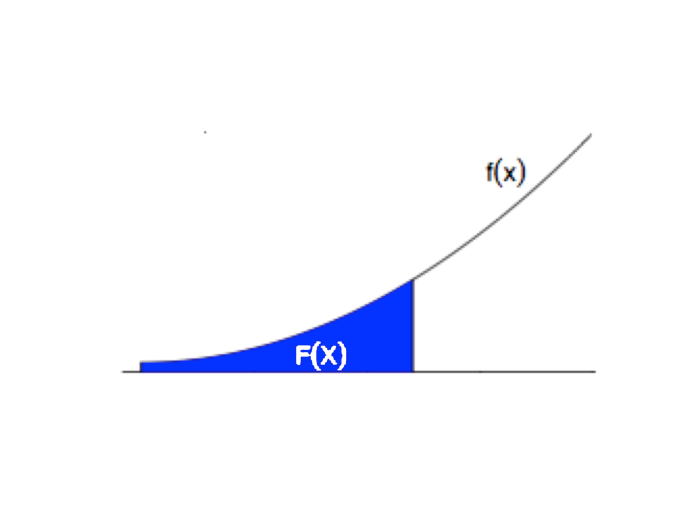
\includegraphics[width=0.55\linewidth]{graficadensidad3}
\end{center}
\vspace*{-2ex}

\blue{A partir d'ara, només considerarem v.a. contínues que tenen funció de densitat}
\end{frame}




\begin{frame}
\frametitle{Propietats}
Si $X$  és una v.a. contínua amb funció de distribució $F_X$ i densitat $f_X$:
\medskip

\begin{itemize} 
\item $F_{X}$ és contínua
\smallskip

\item El \emph{domini} de $X$ és $\emph{D_X}:=\{x\mid f_X(x)>0\}$
\smallskip

\item Si  $A$ és un interval (de qualsevol tipus) amb extrems $a<b$, aleshores $P(X\in A)=\int_a^b f_X(x)\, dx$
\smallskip

Per exemple
$$
\begin{array}{l}
\displaystyle P(a<X\leq b)=P(X\in ]a,b])=\int_{a}^b f_X(x)\, dx\\[2ex]
\displaystyle P(a\leq X)=P(X\in [a,\infty[)=\int_{a}^\infty f_X(x)\, dx
\end{array}
$$
\end{itemize}
\end{frame}

\begin{frame}
\frametitle{Exemple}

La v.a. que ens dóna un nombre escollit a l'atzar dins $]0,1[$ té distribució
$$
F_X(x)=\left\{\begin{array}{ll} 0 &\mbox{ si } x\leq 0 \\
x  & \mbox{ si } 0<x<1\\
1 & \mbox{ si } x\geq 1
 \end{array}\right.
$$
La seva densitat és
$$
f_X(x)=\left\{\begin{array}{ll} 1 &\mbox{ si } 0 <x<1 \\
0 & \mbox{ si $x\leq 0$ o $x\geq 1$ } 
 \end{array}\right.
$$
perquè
$$
F_X(x)=\int_{-\infty}^x f_X(t)\, dt
$$
\end{frame}

%%%%%%%%%

\begin{frame}
\frametitle{Exemple}
\vspace*{-2ex}

En efecte:

\begin{itemize}
    \item Si $x\leq 0$, aleshores 
    $$
    F_X(x)=
\int_{-\infty}^{x}
    0\, dt =0
    $$
    \item Si $0<x<1$, aleshores
$$
\hspace*{-1cm}    F_X(x)=  \int_{-\infty}^{0}
    0\, dt+\int_{0}^{x} 1\, dt = 0+
    \Big[t\Big]_{0}^{x}=x
$$
\item  Si $x\geq 1$, aleshores 
$$
    F_X(x) = \int_{-\infty}^{0}
    0\, dt+\int_{0}^{1} 1\, dt+ \int_1^x 0\,dt= 0+1+0=1
$$


\end{itemize}
\end{frame}







\begin{frame}
\frametitle{Exercici}

\blue{Sigui $X$ una v.a. contínua  amb densitat
$$
f_X(x)=\left\{\begin{array}{ll}
kx^2+\frac{1}{3} & \mbox{ si } 0<x<1\\
0 & \mbox{ si $x\leq 0$ o $x\geq 1$}
\end{array}
\right.$$
amb $k\in \RR$.} 
\medskip

\blue{(a) Què val $k$?}
\medskip

\blue{(b) Qui és $F_X$?}
\medskip

\blue{(c) Què val $P(0.2\leq X\leq 1.2)$?}
\medskip

\blue{(d) Què val $P(X=0.2)$?}
\end{frame}

\begin{frame}
\frametitle{Exercici}
\vspace*{-1ex}

$$
f_X(x)=\left\{\begin{array}{ll}
kx^2+\frac{1}{3} & \mbox{ si } 0<x<1\\
0 & \mbox{ si $x\leq 0$ o $x\geq 1$}
\end{array}
\right.$$
Perquè sigui densitat:
$$
\begin{array}{rl}
\red{1}& \displaystyle \hspace*{-1ex}\red{=\int_{-\infty}^\infty f_X\,dx}\pause =\hspace*{-1ex}\int_{-\infty}^0 \hspace*{-1ex}0\,dx+\int_{0}^1 \Big(k x^2+\frac{1}{3}\Big)\, dx+\int_{1}^\infty \hspace*{-1ex}0\,dx\\[2ex] & \displaystyle \hspace*{-1ex}= 0+\Big[k\frac{x^3}{3}+\frac{1}{3}x\Big]_{0}^{1}+0 = k\frac{1}{3}+\frac{1}{3}
\end{array}
$$
i per tant 
$$1=\dfrac{k+1}{3}\Rightarrow k=2$$
\end{frame}


\begin{frame}
\frametitle{Exercici}
\vspace*{-1ex}
$$
f_X(x)=\left\{\begin{array}{ll}
2x^2+\frac{1}{3} & \mbox{ si } 0<x<1\\
0 & \mbox{ si $x\leq 0$ o $x\geq 1$}
\end{array}
\right.$$
Distribució?
\only<1>{
$$
F_X(x)=\int_{-\infty}^x f_X(t)\, dt
$$
\begin{center}
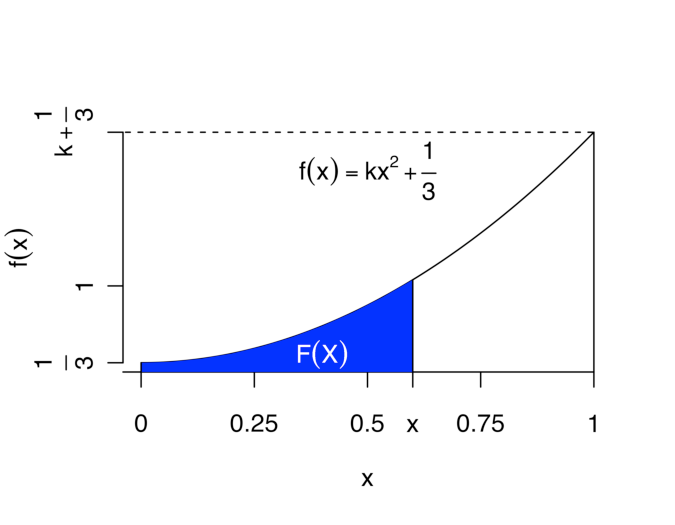
\includegraphics[width=0.8\linewidth]{graficadensidad}
\end{center}}


\only<2>{\begin{itemize}\item \blue{$x\leq 0$}: $$\displaystyle F_X(x)=\int_{-\infty}^x f_X(t)\, dt=\int_{-\infty}^x 0\, dt=0$$\end{itemize}}

\only<3>{\begin{itemize}\item \blue{$0\leq x\leq 1$}:  $$\hspace*{-1cm}\begin{array}{rl}
F_X(x) & \displaystyle =\int_{-\infty}^x \hspace*{-1ex}f_X(t)\, dt=\int_{-\infty}^0 \hspace*{-1ex}0\, dt+\int_{0}^x \Big(2 t^2+\frac{1}{3}\Big)\,  dt\\[2ex] & \displaystyle =0+\Big[2\frac{t^3}{3}+\frac{1}{3}t\Big]_{0}^{x}=2\frac{x^3}{3}+\frac{1}{3}x=\frac{2x^3+x}{3}
\end{array}$$\end{itemize}}


\only<4>{\begin{itemize}\item \blue{$1\leq x$}:  $$\begin{array}{rl}
F_X(x) & \displaystyle =\int_{-\infty}^x f_X(t)\, dt\\[2ex] & \displaystyle=\int_{-\infty}^0 0\, dt+\int_{0}^1 \Big(2 t^2+\frac{1}{3}\Big)\,  dt+\int_{1}^x 0\, dt\\[2ex] & \displaystyle =0+1+0=1
\end{array}$$\end{itemize}}


\end{frame}

\begin{frame}
\frametitle{Exercici}
\vspace*{-1cm}

$$
f_X(x)=\left\{\begin{array}{ll}
2 x^2+\dfrac{1}{3} & \mbox{ si } 0<x<1\\
0 & \mbox{ si $x\leq 0$ o $x\geq 1$}
\end{array}\right.
$$
\begin{center}
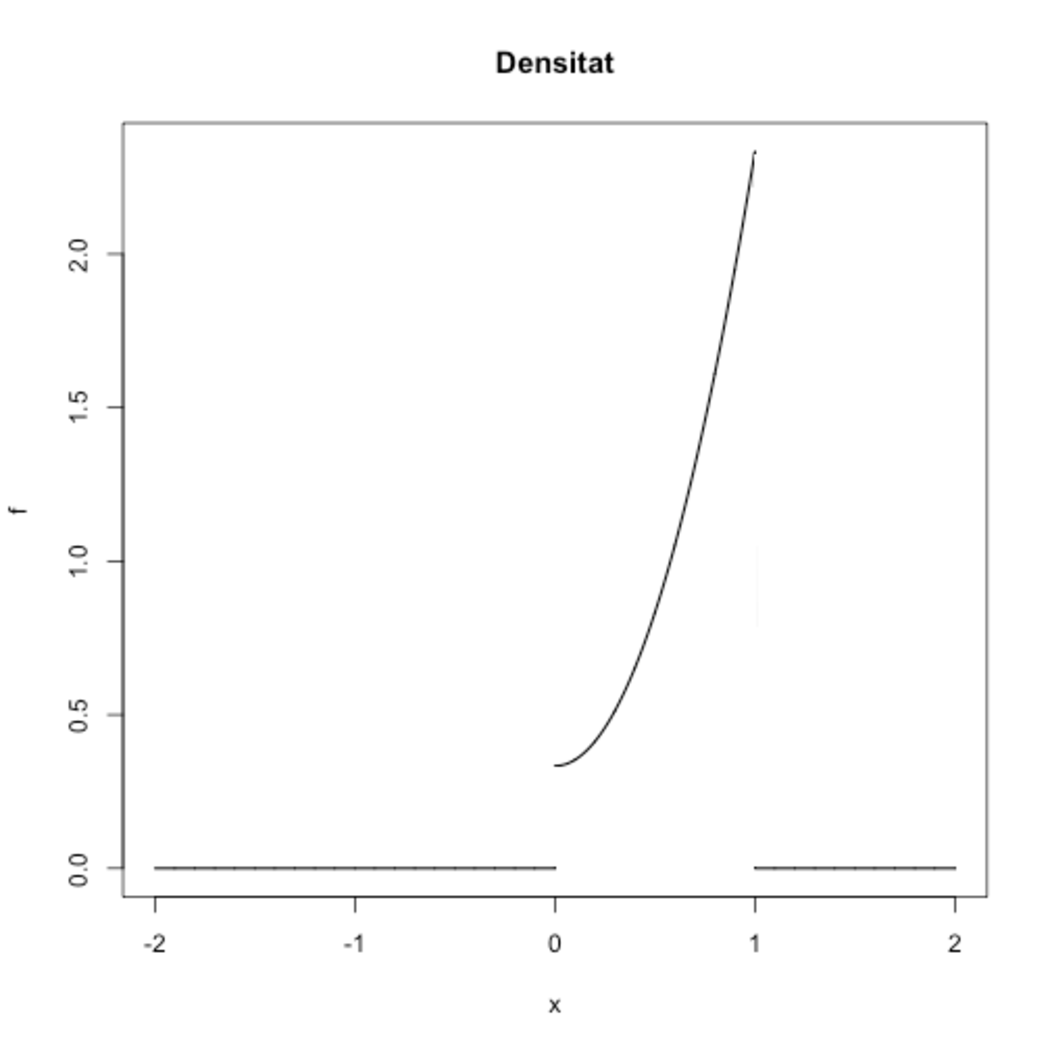
\includegraphics[width=0.7\linewidth]{dens-ex1.pdf}
\end{center}



\end{frame}



\begin{frame}
\frametitle{Exercici}
\vspace*{-1cm}

$$
F_X(x)=\left\{\begin{array}{lll}
0 & \mbox{ si $x\leq 0$}\\
\dfrac{2x^3+x}{3} & \mbox{ si } 0\leq x\leq 1\\
1 & \mbox{ si $x\geq 1$}
\end{array}\right.
$$
\begin{center}
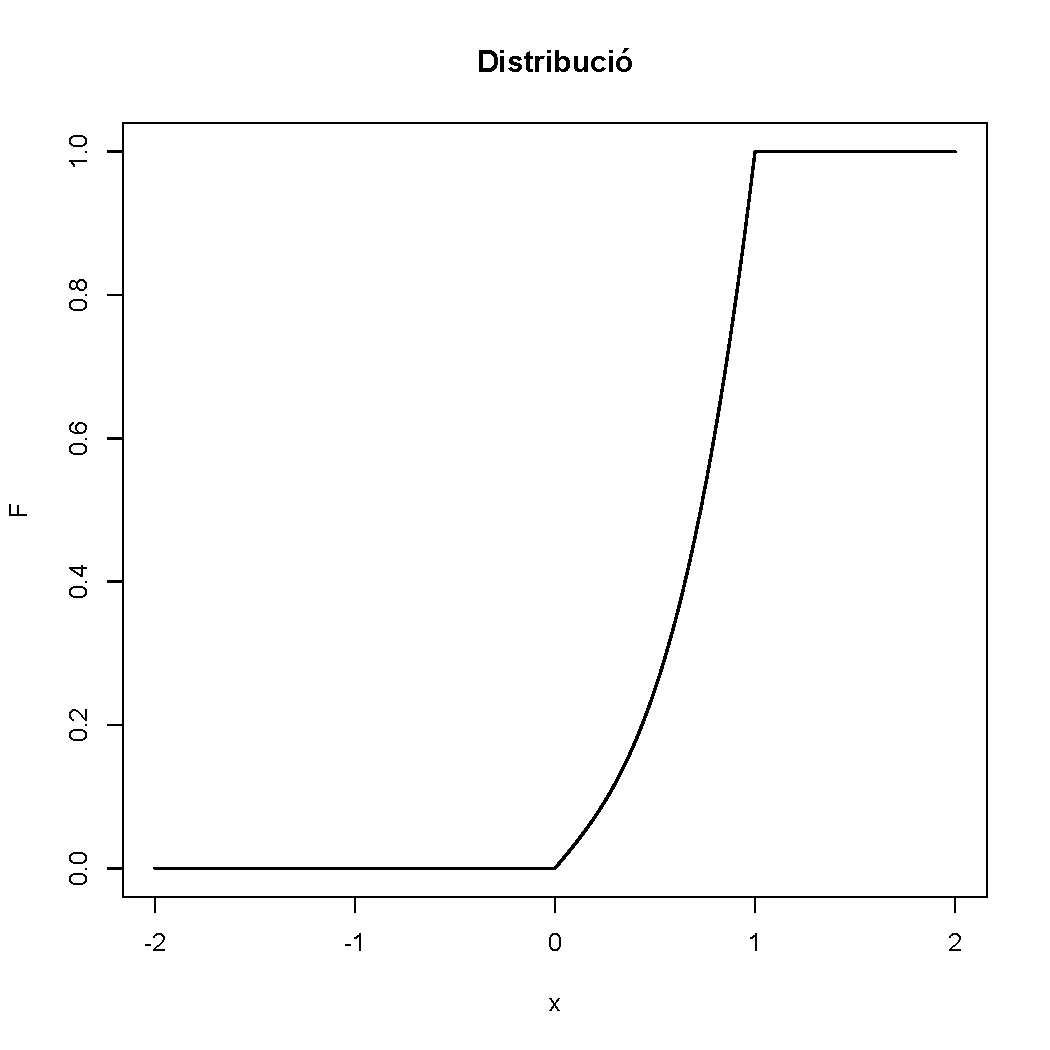
\includegraphics[width=0.7\linewidth]{dist-ex1.pdf}
\end{center}



\end{frame}


\begin{frame}
\frametitle{Exercici}
\vspace*{-1cm}

$$
F_X(x)=\left\{\begin{array}{lll}
0 & \mbox{ si $x\leq 0$}\\
\dfrac{2x^3+x}{3} & \mbox{ si } 0\leq x\leq 1\\
1 & \mbox{ si $x\geq 1$}
\end{array}\right.
$$
\medskip

\blue{$P(0.2\leq X\leq 1.2)$?}\pause
\smallskip

$$
\begin{array}{rl}
P(0.2\leq X\leq 1.2) & =P(X\leq 1.2)-P(X<0.2)\\ & =P(X\leq 1.2)-P(X\leq 0.2)\\ & =F_X(1.2)-F_X(0.2)\\[1ex] & =
1-\dfrac{2\cdot 0.2^3+0.2}{3}=0.928
\end{array}
$$
\pause\medskip

\blue{$P(X=0.2)$?}\pause\ $P(X=0.2)=0$ perquè $X$ és contínua



\end{frame}


\subsection{Esperança i variància}

\begin{frame}
\frametitle{Esperança d'una v.a. contínua}
Sigui $X$ una v.a. contínua amb densitat $f_X$
\medskip

L'\emph{esperança} (\emph{mitjana}, \emph{valor esperat})  de  $X$ és 
$$
E(X)=\int_{-\infty}^{\infty}x \cdot f_{X}(x)\, dx
$$

Si el  domini $D_X$ de $X$ és  un interval amb extrems $a<b$,
$$
E(X)=\int_{a}^{b}x \cdot f_{X}(x)\, dx
$$ 
Sovint també indicarem $E(X)$ amb $\mu$
\medskip

$E(X)$ ``és'' (quasi segurament) el límit de la mitjana dels valors de $X$ si efectuam l'experiment  $n$ vegades i fem $n\to \infty$
\end{frame}

\begin{frame}
\frametitle{Exemple}
Considerem  la v.a. $X$  amb funció de densitat:
$$
f_X(x)=\left\{\begin{array}{ll} 2 x^2+\frac{1}{3} &\mbox{ si $0 <x<1$} \\
0 & \mbox{ si $x\leq 0$ o $x\geq 1$} 
 \end{array}\right.
$$
El seu valor esperat és
$$
\begin{array}{rl}
E(X)= & \displaystyle \int_{0}^1 x \left(2 x^2 +\frac{1}{3}\right)\, dx= \int_{0}^1 \left(2 x^3
+\frac{1}{3}x\right)\, dx\\[3ex] & = \displaystyle
\Big[2 \frac{x^4}{4}+\frac{1}{3} \cdot \frac{x^2}{2}\Big]_{0}^{1}=
 \frac{1}{2}+\frac{1}{6} =\frac{2}{3}
\end{array}
$$

\end{frame}




\begin{frame}
\frametitle{Esperança d'una funció d'una v.a.}

Sigui $X$ una v.a. contínua amb densitat $f_X$ i sigui  $g:D_X\to \RR$ una funció contínua. 
L' \emph{esperança} de la v.a. $g(X)$ és
$$
E(g(X))=\int_{-\infty}^{+\infty} g(x) f_X(x)dx
$$
Si el  domini $D_X$ de $X$ és  un interval amb extrems $a<b$, aleshores
$$
E(g(X))=\int_{a}^{b} g(x) f_X(x)dx
$$
\end{frame}


\begin{frame}
\frametitle{Exemple}
Considerem  la v.a. $X$  amb funció de densitat:
$$
f_X(x)=\left\{\begin{array}{ll} 2 x^2+\frac{1}{3} &\mbox{ si $0 <x<1$} \\
0 & \mbox{ si $x\leq 0$ o $x\geq 1$} 
 \end{array}\right.
$$
El valor esperat de la v.a. $Y=X^2$ és
$$
\begin{array}{rl}
E(Y)& \displaystyle = E(X^2)=\int_{0}^1 x^2 \left(2 x^2 +\frac{1}{3}\right)\, dx\\[3ex] & \displaystyle = \int_{0}^1
\left(2 x^4 +\frac{1}{3}x^2\right)\, dx =
\Big[2 \frac{x^5}{5}+\frac{1}{3}\cdot
\frac{x^3}{3}\Big]_{0}^{1}\\[3ex] & \displaystyle =\frac{2}{5}+\frac{1}{9}=\frac{23}{
45}
\end{array}
$$

\end{frame}


\begin{frame}
\frametitle{Variància d'una v.a. contínua}

Com al cas  discret, la \emph{variància} d'una v.a. contínua $X$ és
$$
Var(X)=E((X-E(X))^2)
$$
i es pot demostrar que
$$
Var(X)=E(X^2)-E(X)^2
$$
Sovint també indicarem la variància amb $\sigma^2$ 
\medskip

La \emph{desviació típica} d'una v.a. $X$ és $\sigma=\sqrt{Var(X)}$
\bigskip

La variància i la desviació típica mesuren com de variats  són els resultats de l'experiment (respecte del valor mitjà)
\end{frame}

\begin{frame}
\frametitle{Exemple}
Considerem  la v.a. $X$  amb funció de densitat:
$$
f_X(x)=\left\{\begin{array}{ll} 2 x^2+\frac{1}{3} &\mbox{ si $0 <x<1$} \\
0 & \mbox{ si $x\leq 0$ o $x\geq 1$} 
 \end{array}\right.
$$
Ja hem calculat 
$$E(X)=\frac{2}{3},\quad E(X^2)=\frac{23}{45}
$$
Per tant
$$
Var(X)=E(X^2)-E(X)^2= \frac{23}{45}-\left(\frac{2}{3}\right)^2=\frac{1}{15}
$$
\end{frame}


 \begin{frame}
\frametitle{Propietats}
Tenim les mateixes propietats que en el cas discret:
\begin{enumerate}[a)]
\item $E(a)=a$, on $a$ és una constant real
\smallskip

\item $E(a X+b)=a E(X)+b$
\smallskip

\item $ E\left(X+Y\right)=E(X)+E(Y)$
\smallskip

\item Si $a<X<b$, aleshores $a<E(X)<b$
\smallskip

\item Si $X\geq 0$, aleshores $E(X)\geq 0$
\smallskip

\item Si $g(X)\leq h(X)$, aleshores $E(g(X))\leq E(h(X))$
\smallskip

\item $Var(aX+b)=a^2 Var(X)$, on $a,b$ són constants reals
\smallskip

\item $Var(a)=0$, on $a$ és una constant real
\smallskip

\item $Var(X+Y)=Var(X)+Var(Y)$ si $X,Y$ són independents
\end{enumerate}
\end{frame}


%\begin{frame}
%\frametitle{Exemple}
%
%\blue{Sigui $X$ una v.a. contínua amb densitat
%$$
%f(x) = \left\{\begin{array}{ll}  k (1+x^2) & \mbox{ si $x   \in ]0,3[$}\\ 
%0  & \mbox{ si $x   \notin ]0,3[$}\end{array}\right.
%$$
%amb $k\in \RR$}
%\begin{itemize} 
%\item \blue{Què val la constant $k$?}
%\item \blue{Quina és la distribució $F_X$ de $X$?}
%\item \blue{Calculau $P(X=1.5)$}
%\item \blue{Calculau $P(1\leq X\leq 2)$}
%\item \blue{Què val $E(X)$? Què val $\sigma(X)$?}
%\end{itemize}
%%\sol{a)$\mathbf{k=1/12}$; b) $\mathbf{5/18}$; 
%
%\end{frame}
%

\section{Algunes distribucions contínues}

\subsection{Distribució  uniforme}

\begin{frame}[fragile]
\frametitle{Distribució uniforme}
Una v.a. contínua $X$ té \emph{distribució uniforme}
sobre l'interval real
$]a,b[$ ($a<b$), i ho indicarem amb \emph{$U(a,b)$}, si la seva funció de densitat és
 $$
 f_X(x)=
 \left\{\begin{array}{ll}
\dfrac{1}{b-a} & \mbox{si } a<x<b\\[2ex] 0  & \mbox{si $x\leq a$ o $x\geq b$}
\end{array}
\right. $$ 
Una variable $U(a,b)$ modela el triar un element dins $]a,b[$ de manera equiprobable
\medskip

Amb {\tt R}, és \texttt{unif}

\end{frame}


\begin{frame} 
\frametitle{Distribució uniforme}
 $U(1,5):\quad f_X(x)=
 \left\{\begin{array}{ll}
\dfrac{1}{4} & \mbox{si } 1<x<5\\[2ex] 0  & \mbox{si $x\leq 1$ o $x\geq 5$}
\end{array}
\right. $

\begin{center}
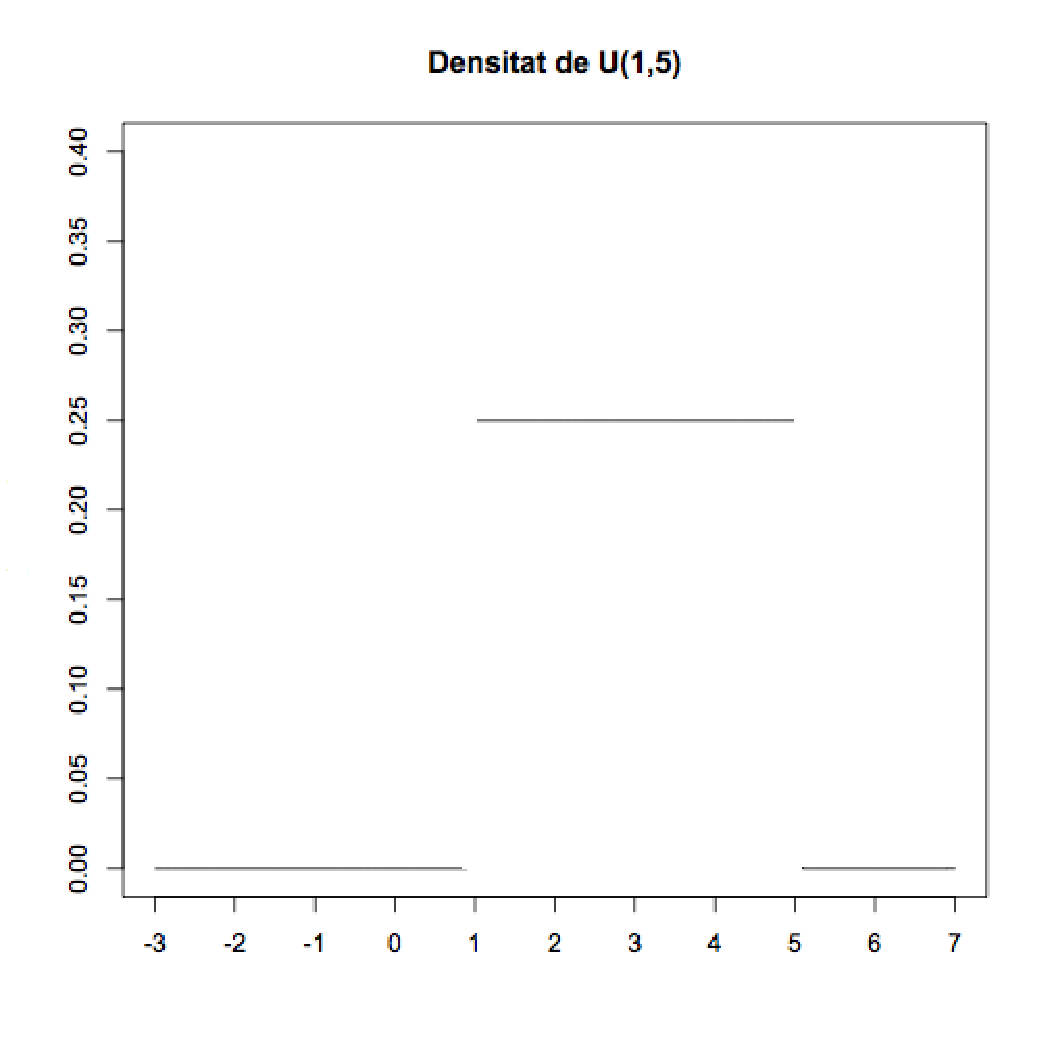
\includegraphics[width=0.6\linewidth]{dunif15}
\end{center}



\end{frame}


 
\begin{frame} 
\frametitle{Distribució uniforme}
\vspace*{-1ex}

Integrant, la funció de distribució surt:
$$
F_X(x)=\left\{\begin{array}{ll} 0  & \mbox{si } x\leq a\\
\dfrac{x-a}{b-a} & \mbox{si } a<x<b\\ 1  & \mbox{si } b\leq x
\end{array}
\right. 
$$
\vspace*{-3ex}

\begin{center}
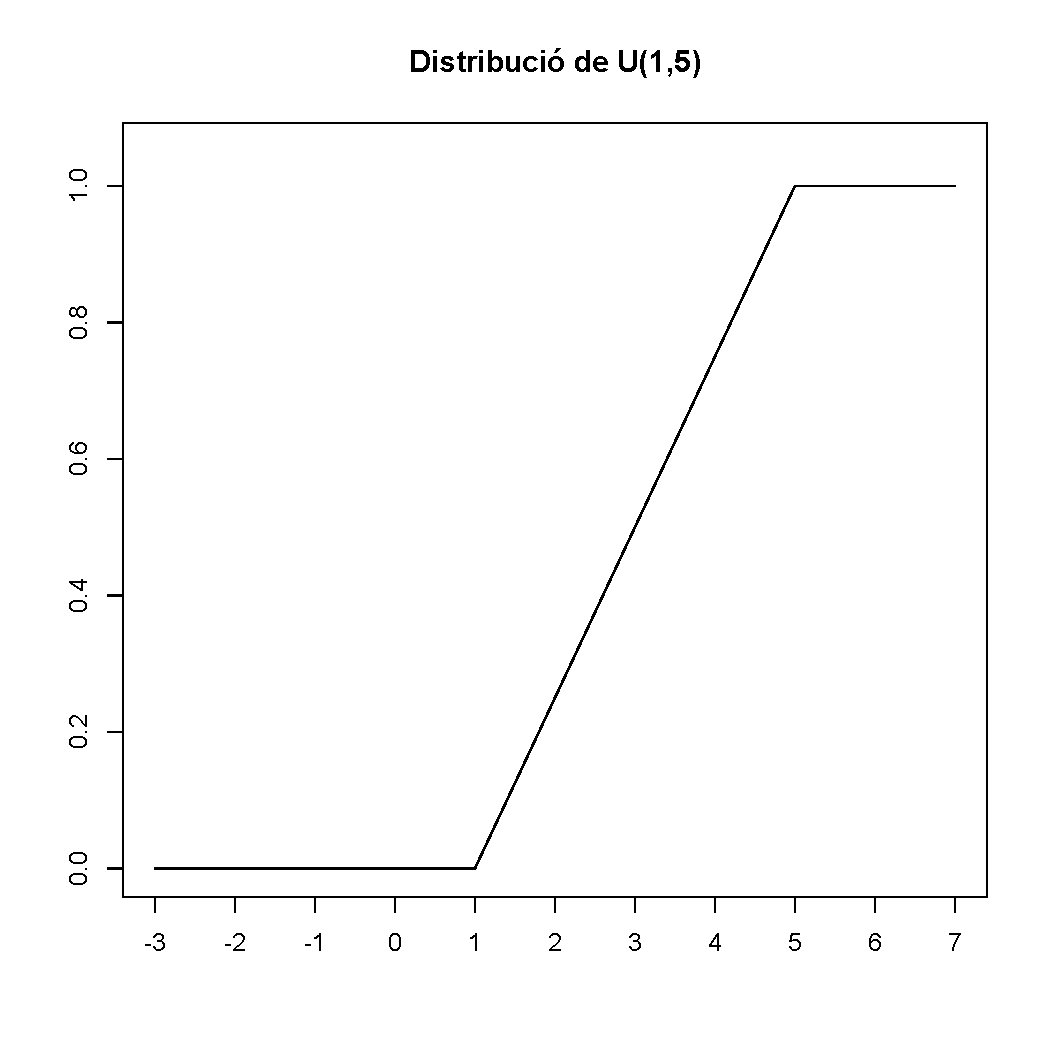
\includegraphics[width=0.625\linewidth]{punif15}
\end{center}



\end{frame}


\begin{frame}
\frametitle{Resum de propietats}
\vspace*{-2ex}

 Sigui $X$ una v.a. $U(a,b)$.
 \medskip
 
\begin{itemize}
\item  Domini: $D_X=]a,b[$
\medskip

\item Densitat: $f_X(x)=\left\{\begin{array}{ll}
\dfrac{1}{b-a} & \mbox{si } a<x<b\\ 0  & \mbox{ si $x\leq a$ o $x\geq b$}
\end{array} \right.$
\medskip

\item Distribució: $F_X(x)=\left\{\begin{array}{ll} 0 & \mbox{ si } x\leq a\\
          \dfrac{x-a}{b-a} & \mbox{ si } a\leq x\leq b\\
          1 & \mbox{ si } b\leq x\end{array}\right.$
 \medskip
         
\item Esperança: $E(X)= \dfrac{a+b}{2}$
\medskip

\item Variància: $Var(X)=\dfrac{(b-a)^2}{12}$
\end{itemize}

\end{frame}



\begin{frame}
\frametitle{Esperança i variància}
\vspace*{-2ex}

Sigui $X$ una v.a. $U(a,b)$
\vspace*{-3ex}

\begin{eqnarray*}
\red{E(X)} &\hspace*{-1ex}= & \hspace*{-2ex}\int_{-\infty}^{+\infty} \hspace*{-3ex}x \cdot f_X(x)\, dx=\int_{a}^{b} \hspace*{-1ex}x \frac{1}{b-a}\, dx \\ &\hspace*{-2ex}= & \hspace*{-2ex}
\Big[\frac{x^2}{2(b-a)}\Big]_{a}^{b}=\red{\frac{b+a}{2}} \\[2ex] 
E(X^2)& \hspace*{-1ex}=  & \hspace*{-2ex} \int_{-\infty}^{+\infty} \hspace*{-3ex} x^2\cdot f_X(x)\, dx=\int_{a}^{b}  \hspace*{-1ex}x^2 \frac{1}{b-a}\, dx \\ &\hspace*{-2ex}= & \hspace*{-2ex}\Big[\frac{x^3}{3(b-a)}\Big]_{a}^{b} =\frac{b^3-a^3}{3(b-a)} = \frac{b^2+ab+a^2}{3} \\ 
\red{Var(X)} & \hspace*{-1ex}= & \hspace*{-1ex} E(X^2)-(E(X))^2=\frac{b^2+ab+a^2}{3}-\left(\frac{b+a}{2}\right)^2\\ & \hspace*{-1ex}= & \hspace*{-1ex} \red{\frac{(b-a)^2}{12}}
\end{eqnarray*}
\end{frame}

%\begin{frame}
%\frametitle{Exemple}
%
%Tenim una espècie de plantes angiospermes, les flors de la qual no demostren cap preferència en la seva orientació, i per tant cada flor admet totes les orientacions amb la mateixa probabilitat\bigskip
%
%
%Si mesuram l'orientació en graus, amb el 0 a l'est i en sentit antihorari, podem considerar que la v.a. $X$ que dóna aquesta orientació és $U(0,360)$
%\medskip
%
%Densitat: $f_X(x)=\left\{\begin{array}{ll}
%\dfrac{1}{360} & \mbox{si } 0<x<360\\[2ex] 0  & \mbox{ si $x\leq 0$ o $x\geq 360$}
%\end{array} \right.$
%
%\end{frame}
%
%\begin{frame}
%\frametitle{Exemple}
%
%
%\blue{Quina és la probabilitat que una flor estigui orientada exactament a nord ($90^{\mathrm{o}}$)?}
%\medskip
%\pause
%
%$\displaystyle P(X=90)=0$
%\bigskip
%\pause
%
%
%\blue{Quina és la probabilitat que una flor estigui orientada a nord, amb un error de menys de $5^{\mathrm{o}}$?}
%\medskip
%\pause
%
%$\displaystyle P(85<X<95)=\int_{85}^{95}\frac{1}{360}\,dt=\Big[\frac{t}{360}\Big]_{85}^{95}=\frac{10}{360}=\frac{1}{36}$
%\bigskip
%\pause
%
%\blue{Quina és la desviació típica de les orientacions de les flors?}
%\medskip
%\pause
%
%$\displaystyle \sigma=\sqrt{\frac{360^2}{12}}=\frac{360}{\sqrt{12}}\approx 103.9^{\mathrm{o}}$
%
%
%
%\end{frame}
%



\subsection{Distribució  normal}

\begin{frame}
\frametitle{Distribució normal}
Una v.a. $X$ segueix una \emph{llei normal} o \emph{gaussiana} de
paràmetres $\mu$ i $\sigma$, i ho indicarem amb \red{$N(\mu,\sigma)$}, quan té funció de densitat $$
f_{X}(x)=\frac{1}{\sqrt{2\pi}\sigma} e^{{-(x-\mu)^2}/{(2\sigma^{2})}} \mbox{
per a tot } x\in \RR
$$
\bigskip

Quan $\mu=0$ i $\sigma=1$, direm que la v.a. normal és \emph{estàndard}, i la indicarem usualment $Z$
$$
f_{Z}(x)=\frac{1}{\sqrt{2\pi}} e^{ -x^2/2} \mbox{
per a tot } x\in \RR
$$

Amb R, és \texttt{norm}
\end{frame}

\begin{frame} 
\frametitle{Distribució normal}

La gràfica de $f_X$ és la coneguda \emph{campana de Gauss}
\begin{center}
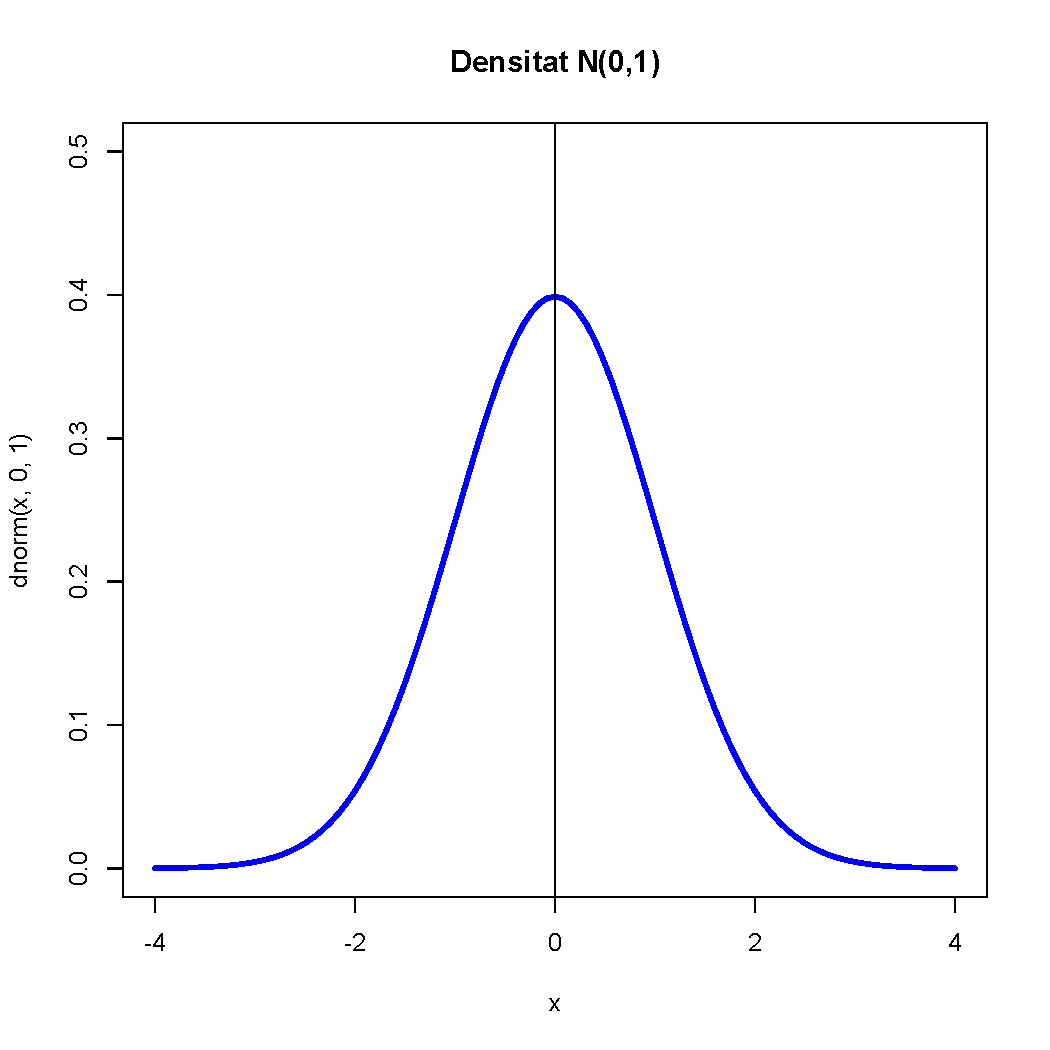
\includegraphics[width=0.8\linewidth]{dnorm01}
\end{center}

\end{frame}


\begin{frame} 
\frametitle{Distribució normal}



La distribució normal és una de les més importants en estadística, perquè aproxima molt bé molts fenòmens naturals:
\medskip

\begin{itemize}
\item Alçades, inte\l.ligència,\ldots
\item Notes, encerts, errors de mesura, \ldots
\end{itemize}

A més, 
\begin{itemize}
\item Moltes variables aleatòries consistents en prendre una mostra de $N$ elements i calcular qualque cosa (per exemple, la mitjana) tenen distribució aproximadament normal quan $N$ és gran, encara que la distribució dels elements individuals no ho sigui
\end{itemize}


\end{frame}


\begin{frame}
\frametitle{Propietats} 
\vspace*{-1ex}

Sigui $X$ una v.a. $N(\mu,\sigma)$
\medskip

\begin{itemize}
\item $f_X$ és simètrica respecte de $x=\mu$:
$$
f_{X}(\mu-x)=f_{X}(\mu+x)
$$
i té el màxim a $x=\mu$
\medskip

En particular, si $Z$ es una $N(0,1)$, aleshores
$f_{Z}(-x)=f_{Z}(x)$, i $f_Z$ pren el valor màxim a $x=0$
\end{itemize}
\vspace*{-5ex}

\begin{center}
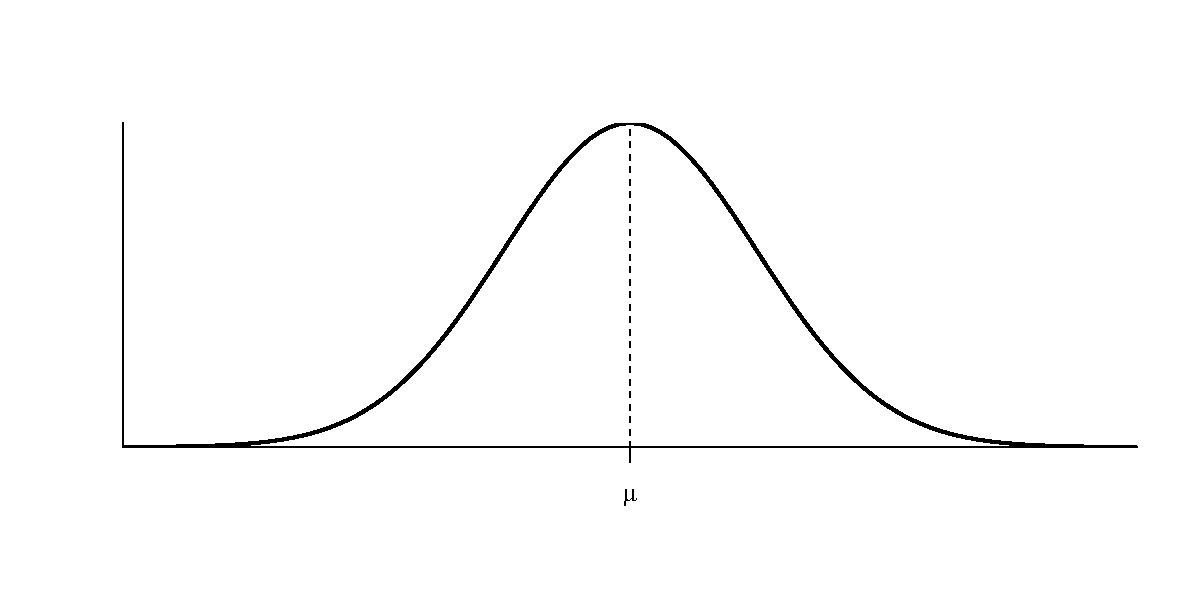
\includegraphics[width=\linewidth]{simn}
\end{center}
\end{frame}

%
%\begin{frame}
%\frametitle{Propietats} 
%
%Recordem que $P(X\leq x)=F_X(x)$ és l'àrea compresa entre $f_X$, l'eix $y=0$ i la recta vertical a $x$
%\begin{center}
%\includegraphics[width=\linewidth]{undernorm}
%\end{center}
%\end{frame}
%

\begin{frame}
\frametitle{Propietats} 
\begin{itemize}
\item Aquesta simetria fa iguals les àrees a l'esquerra de $\mu-x$ i a la dreta de $\mu+x$

\begin{center}
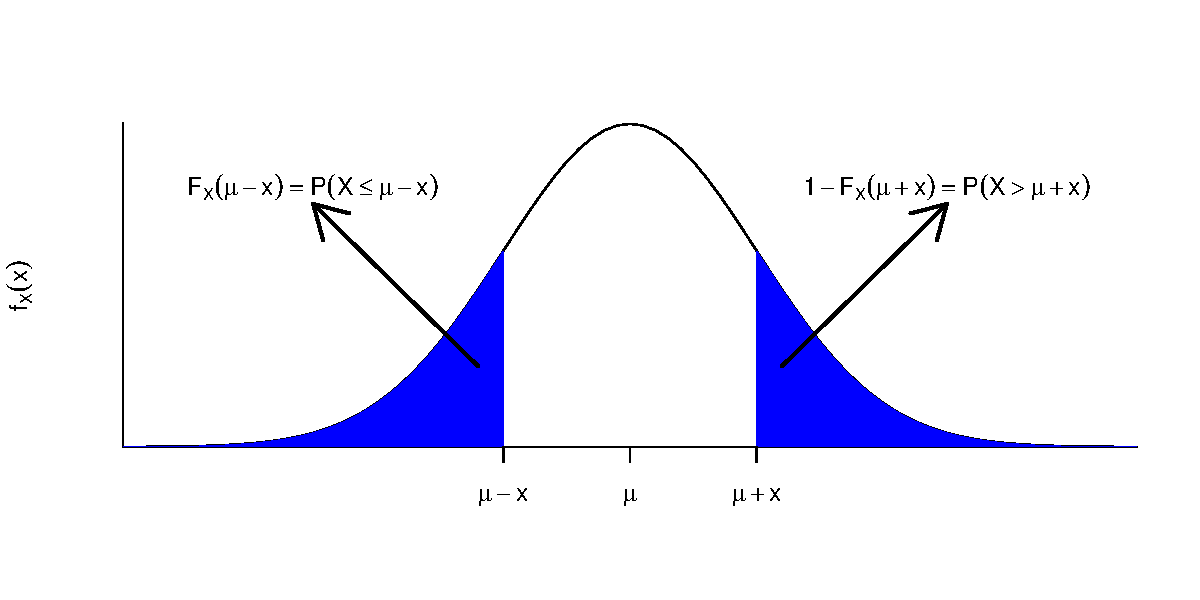
\includegraphics[width=\linewidth]{simnorm1}
\end{center}
\vspace*{-1.5cm}

$$
\begin{array}{rl}
\red{F_{X}(\mu-x)} & =P(X\leq \mu-x)\\ &
=P(X\geq \mu+x) \red{{} =1-F_{X}(\mu+x)}
\end{array}
$$
\end{itemize}
\end{frame}


\begin{frame}
\frametitle{Propietats} 
\begin{itemize}
\item A $N(0,1)$, aquesta simetria fa iguals  les àrees a l'esquerra de $-z$ i a la dreta de $z$
\begin{center}
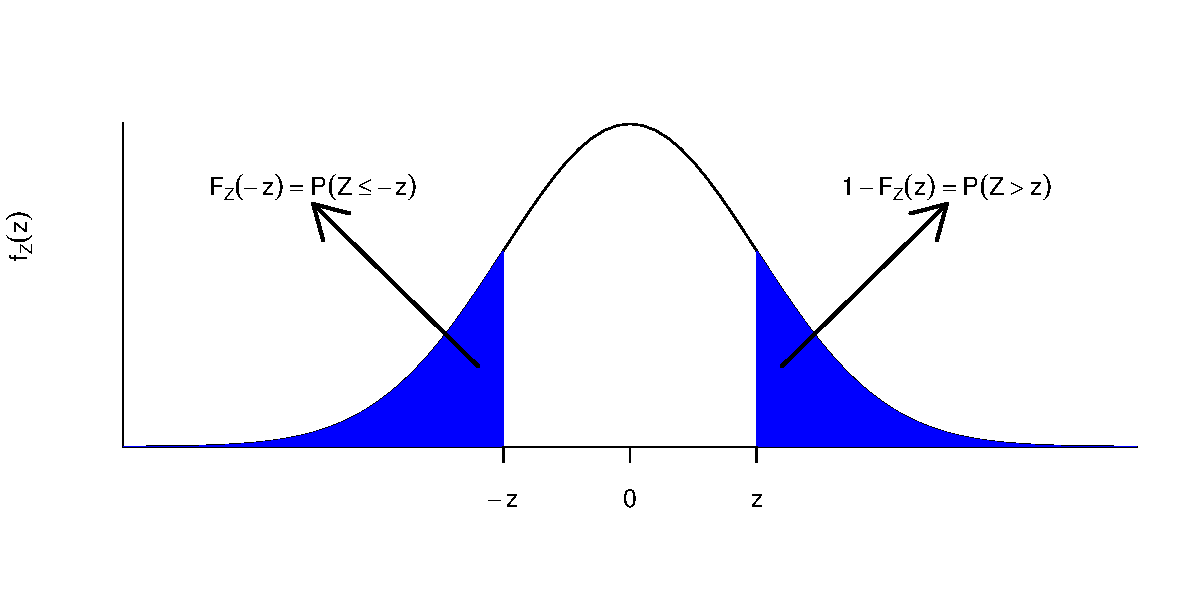
\includegraphics[width=\linewidth]{simnorm2}
\end{center}
\vspace*{-1cm}

$$
\red{F_{Z}(-z)}=P(Z\leq -z)=P(Z\geq  z)\red{{} =1-F_{Z}(z)}
$$
\end{itemize}
\end{frame}

\begin{frame}
\frametitle{Propietats} 
Sigui $X$ una v.a. $N(\mu,\sigma)$
\medskip

\begin{itemize}


\item$E(X)=\mu$ 
\medskip

\item$Var(X)=\sigma^2$ 
\medskip

\item  La seva desviació típica és $\sigma$
\end{itemize}
\bigskip

En particular, si $Z$ és una normal estàndard, $E(Z)=0$ i $Var(Z)=1$.
\end{frame}



\begin{frame}
\frametitle{Distribució normal}

Augmentar la $\mu$ desplaça a la dreta el màxim, i amb ell tota la corba
\begin{center}
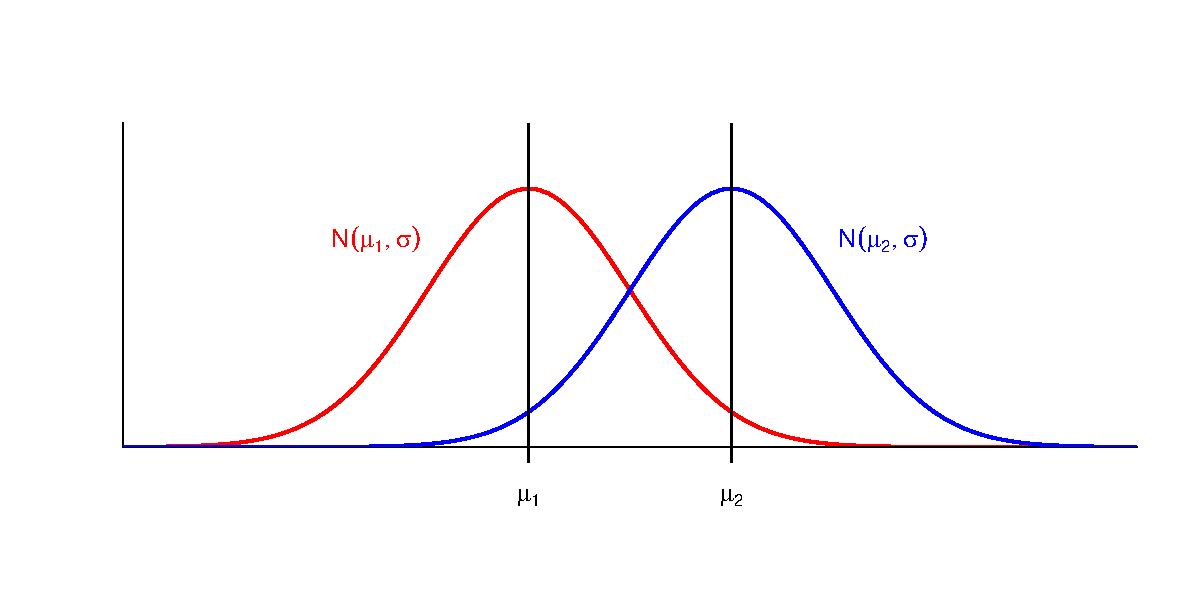
\includegraphics[width=\linewidth]{mu1mu2}

$\mu_1<\mu_2$
\end{center}
\end{frame}




\begin{frame}
\frametitle{Distribució normal}

Augmentar la $\sigma$ aplata la corba: en augmentar la variància, els valors s'allunyen més del valor mitjà
\begin{center}
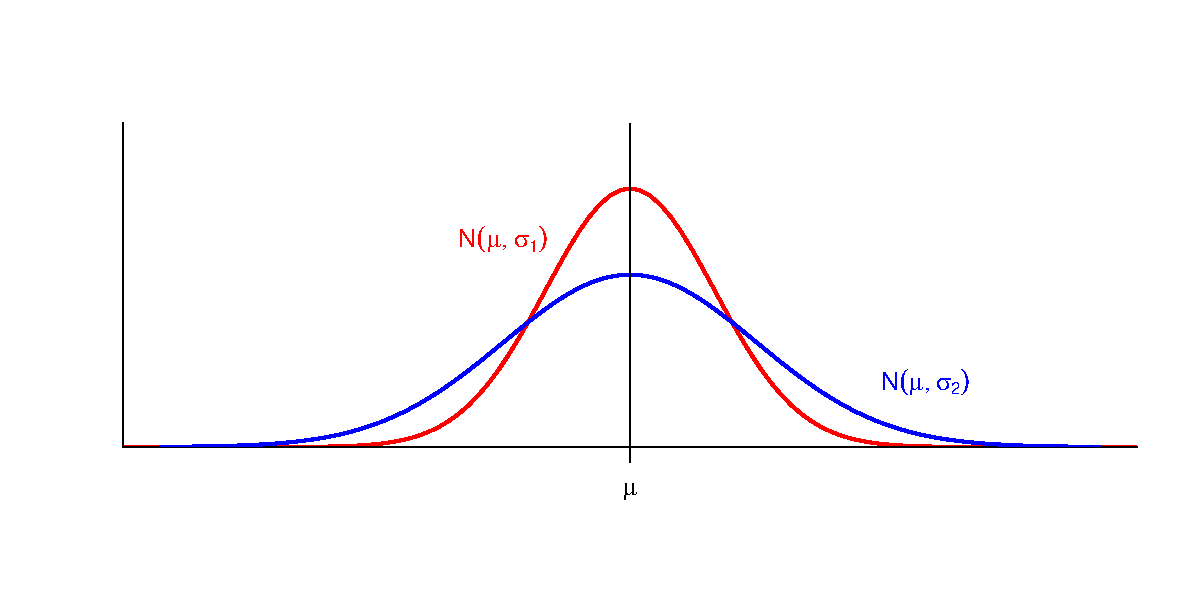
\includegraphics[width=\linewidth]{sigma1sigma2}

$\sigma_1<\sigma_2$
\end{center}
\end{frame}




\begin{frame}
\frametitle{Distribució normal}

L'efecte combinat
\begin{center}
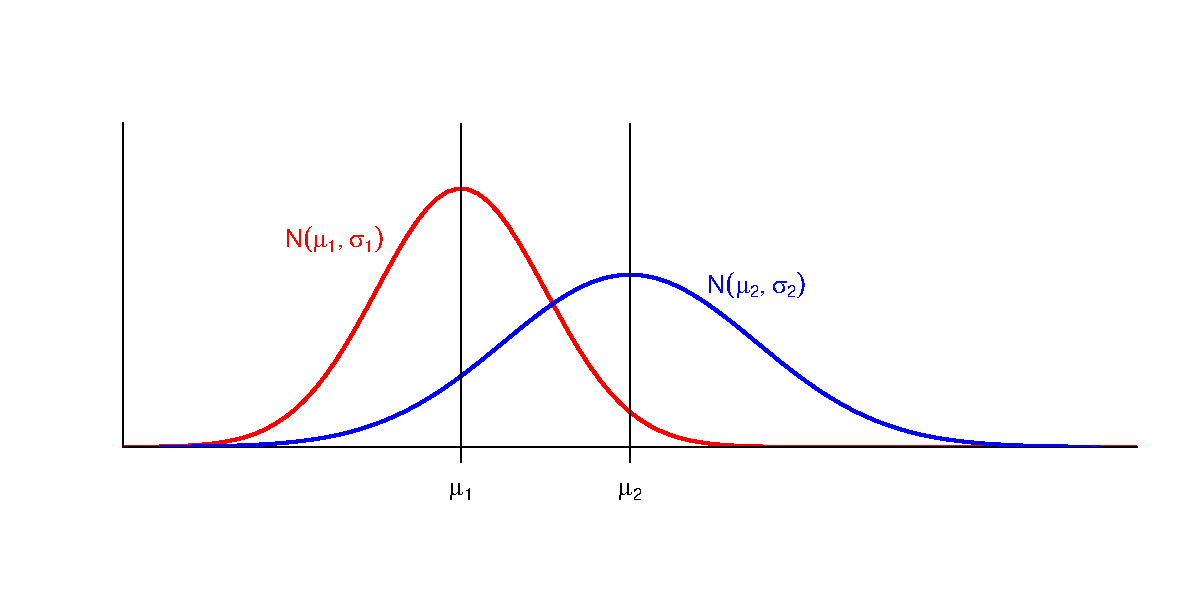
\includegraphics[width=\linewidth]{musigma}

$\mu_1<\mu_2,\ \sigma_1<\sigma_2$
\end{center}
\end{frame}




\begin{frame}
\frametitle{Estandardització d'una v.a.\ normal}

\begin{teorema}
Si $X$ és una v.a. $N(\mu,\sigma)$, aleshores
$Z=\dfrac{X-\mu}{\sigma}$
és $N(0,1)$.
\end{teorema}

Les probabilitats d'una normal estàndard $Z$ determinen les de qualsevol $X$ de tipus $N(\mu,\sigma)$:
$$
\begin{array}{rl}
\red{P(X\leq x)} & \displaystyle \hspace*{-1ex} =P\Big(\frac{X-\mu}{\sigma}\leq \frac{x-\mu}{\sigma}\Big)\red{=P\Big(Z\leq \frac{x-\mu}{\sigma}\Big)}\\[1ex]
\red{P(y\leq X\leq x)} & \displaystyle \hspace*{-1ex} =P\Big( \frac{y-\mu}{\sigma}\leq \frac{X-\mu}{\sigma}\leq \frac{x-\mu}{\sigma}\Big)\\[1ex] & \displaystyle \hspace*{-1ex} \red{=P\Big(\frac{y-\mu}{\sigma}\leq Z\leq \frac{x-\mu}{\sigma}\Big)}
\end{array}
$$
\end{frame}


\begin{frame}
\frametitle{Càlcul de probabilitats}
\vspace*{-2ex}

$F_Z$ no té expressió coneguda. La podeu calcular amb R (\texttt{pnorm}) o altres programes (hi ha Apps per iPhone o Android), o, a mà, amb taules.
Les taules per calcular $F_Z$ són al fitxer \blue{\underline{\texttt{tablasnormal.pdf}}} a Campus Extens.
\vspace*{-2ex}

\begin{center}
\hspace*{-0.4cm}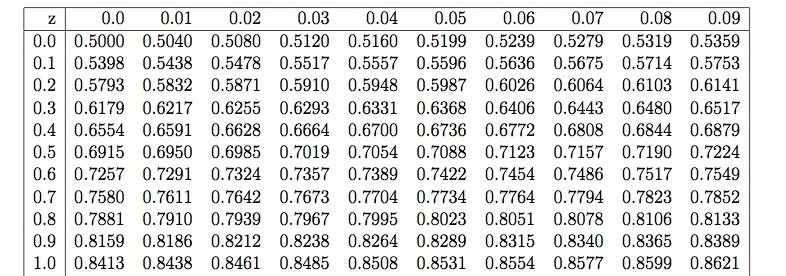
\includegraphics[width=1.1\linewidth]{tabla.jpg}
\end{center}
\pause

{\small $F_Z(0.75)=0.7734,\pause\ F_Z(1.02)=0.8461,\pause\ F_Z(0.06)=\pause 0.5239$\\[1ex]
\pause

$F_Z(-0.75)=1-F_Z(0.75)=0.2266,\pause\ F_Z(-0.88)=\pause 0.1894$

}
\end{frame}


\begin{frame}
\frametitle{Càlcul de probabilitats}
\vspace*{-1cm}

\begin{center}
\hspace*{-0.2cm}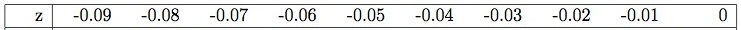
\includegraphics[width=1.06\linewidth]{taula4.jpg}
$$
\vdots
$$
\hspace*{-0.4cm}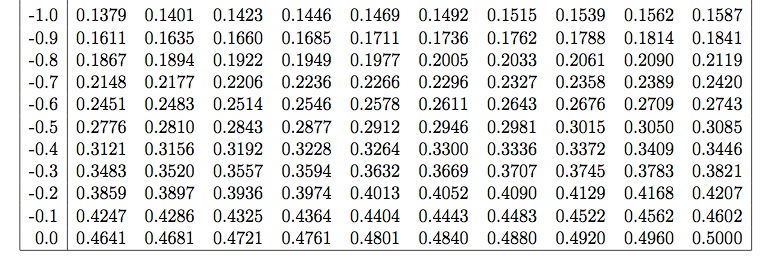
\includegraphics[width=1.1\linewidth]{tabla2.jpg}
\end{center}

{\small 
$F_Z(-0.75)= 0.2266,\ F_Z(-0.88)= 0.1894$

}
\end{frame}



\begin{frame}
\frametitle{Càlcul de probabilitats}
\vspace*{-1cm}

\begin{center}
\hspace*{-0.4cm}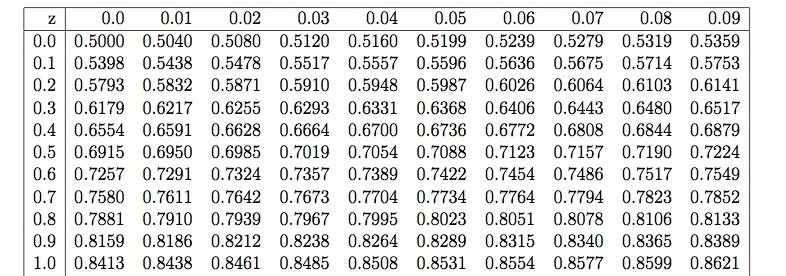
\includegraphics[width=1.1\linewidth]{tabla.jpg}
\end{center}
$$
\begin{array}{rl}
P(0.25<Z<0.75) & =P(Z<0.75)-P(Z<0.25)\\ & =0.7734-0.5987=0.1747\\[2ex]\pause
P(-0.3<Z<0.3) & =\pause P(Z<0.3)-P(Z<-0.3)\\ & =P(Z<0.3)-1+P(Z<0.3)\\ & =2P(Z<0.3)-1=0.2358
\end{array}
$$
\end{frame}


%\begin{frame}
%
%\frametitle{Exemple} 
%Sea $Z$ una variable normal estándar. Utilizando las tablas de la distribución
%normal estándar calcular las siguientes probabilidades:
%\begin{enumerate}[a)]
%\item $P(0< Z < 3.99)=F_Z(3.99)-F_Z(0)\approx 1-0.5=0.5$. 
%\item $P(-3.99\leq Z \leq 3.99)=F_{Z}(3.99)-F_{Z}(-3.99)\approx 1.$
%\item $P(-3\leq Z \leq 3)=F_{Z}(3)-F_{Z}(-3)= 0.9987-0.0013=0.9974$.
%\item $P(Z\leq -2)=F_Z(-2)=0.0228$.
%\item $P( Z \leq 2)=F_{Z}(2)=0.9772$.
%\item $P( Z \geq 2)=1-P(Z<2)=1-F_{Z}(2)=0.0228$.
%\item $P( Z \geq -2)=1-P(Z< -2)=1-F_{Z}(-2)=1-(1-F_Z(2))=F_Z(2)$.
%\item Dado $\delta>0$, $P(-\delta\leq Z \leq
%\delta)=F_{Z}(\delta)-F_{Z}(-\delta)=F_Z(\delta)-(1-F_Z(\delta))=2\cdot 
%F_Z(\delta)-1$.
%\item Utilizando la igualdad anterior
%$P(-2\leq Z \leq 2)=2\cdot  F_Z(2)-1=2 \cdot 0.9772-1=0.9544$.
%\end{enumerate}
%
%\end{frame}


\begin{frame}
\frametitle{Càlcul de quantils}

Les taules també es poden emprar per ``calcular'' quantils (amb R, \texttt{qnorm}).
\medskip

Si volem saber el valor de $z$ tal que $P(Z\leq z)=q$, cercam a la taula l'entrada $q$ (o el més proper) i miram a quin $z$ correspon.
\vspace*{-3ex}

\begin{center}
\hspace*{-0.4cm}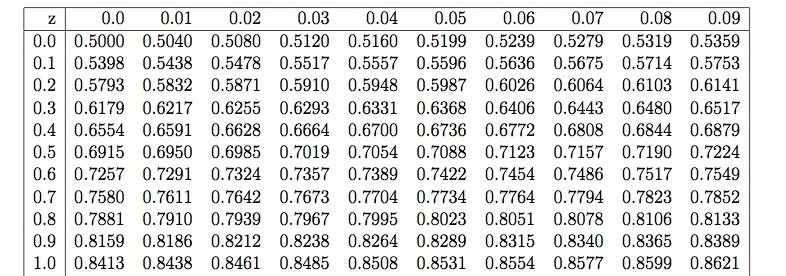
\includegraphics[width=1.1\linewidth]{tabla.jpg}
\end{center}
\vspace*{-2ex}

Quin és el valor $z$ tal que $P(Z\leq z)=0.7357$? $z=0.63$


\end{frame}

\begin{frame}[fragile]
\frametitle{Càlcul de quantils}
\vspace*{-1cm}


\begin{center}
\hspace*{-0.4cm}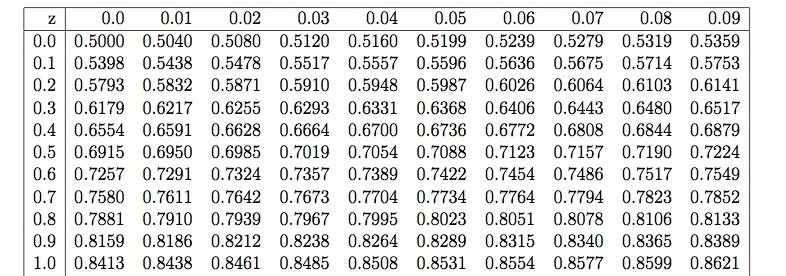
\includegraphics[width=1.1\linewidth]{tabla.jpg}
\end{center}
\vspace*{-2ex}

Quin és el valor $z$ tal que $P(Z\leq z)=0.8357$?\\ \pause Entre 0.97 i 0.98
\begin{verbatim}
> qnorm(0.8357)
[1] 0.9769377
\end{verbatim}

\end{frame}


\begin{frame}
\frametitle{Amb les normals no estàndard\ldots}
\vspace*{-1cm}

\begin{center}
\hspace*{-0.4cm}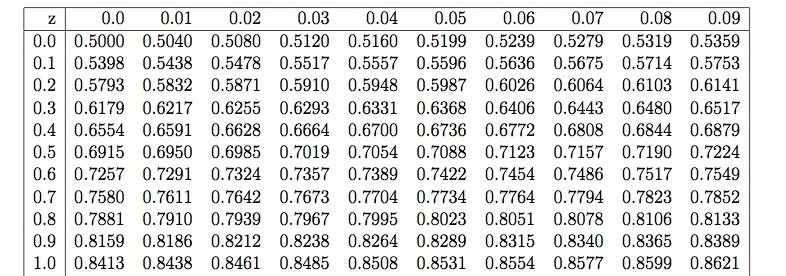
\includegraphics[width=1.1\linewidth]{tabla.jpg}
\end{center}

Sigui $X$ una v.a. $N(1,2)$. Què val $P(X\leq 2)$?
$$
P(X\leq 2)=P\Big(Z\leq\frac{2-1}{2}=0.5\Big)=0.6915
$$

\end{frame}

\begin{frame}
\frametitle{Amb les normals no estàndard\ldots}
\vspace*{-1cm}

\begin{center}
\hspace*{-0.4cm}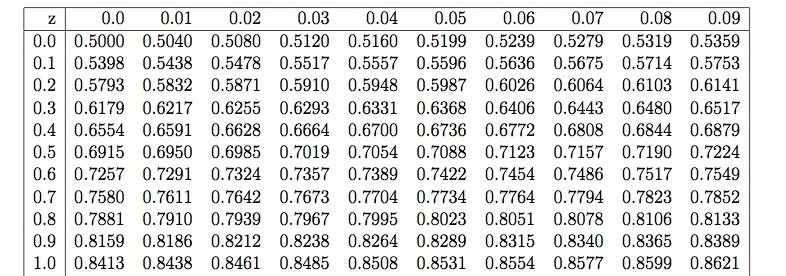
\includegraphics[width=1.1\linewidth]{tabla.jpg}
\end{center}

Sigui $X$ una v.a. $N(1,2)$. Per a quin $x$ es té que $P(X\leq x)=0.7939$?
$$
\begin{array}{l}
0.7939=P(X\leq x)=P\Big(Z\leq\dfrac{x-1}{2}\Big)\\[1ex]\qquad\qquad\qquad\qquad \Rightarrow \dfrac{x-1}{2}=0.82
\Rightarrow x=2.64
\end{array}
$$

\end{frame}

\begin{frame}
\frametitle{Amb les normals no estàndard\ldots}
\vspace*{-1cm}

\begin{center}
\hspace*{-0.4cm}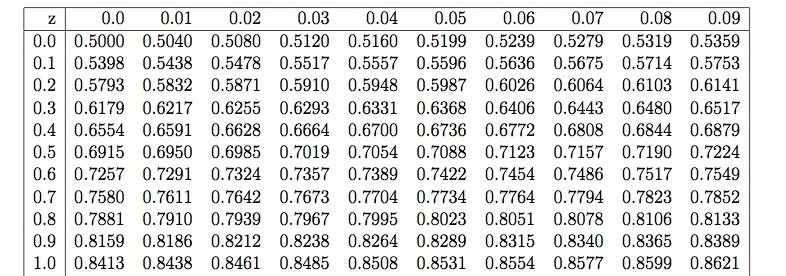
\includegraphics[width=1.1\linewidth]{tabla.jpg}
\end{center}

Sigui $X$ una v.a. $N(0.5,1.5)$. \medskip

Què val $P(X\leq 1.5)$? \medskip

Per a quin $x$ es té que $P(X\leq x)=0.834$?



\end{frame}




\subsection{Distribució exponencial}

\begin{frame}[fragile]
\frametitle{Distribució exponencial}
Una v.a. contínua $X$ té \emph{distribució exponencial} de paràmetre $\lambda$, i ho indicarem amb \emph{$Exp(\lambda)$}, si la seva funció de densitat és
 $$
 f_X(x)=
 \left\{\begin{array}{ll}
0 & \mbox{si } x\leq 0\\[2ex] \lambda e^{-\lambda x}  & \mbox{si $x>0$}
\end{array}
\right. $$ 
És densitat:
$$
\int_0^\infty  \lambda e^{-\lambda t}\,dt=\lim_{x\to\infty}\Big[-e^{-\lambda t}\Big]_0^x=\lim_{x\to\infty}-e^{-\lambda x}+1=1
$$

Amb R és \texttt{exp}
%\begin{verbatim}
%> dexp(3,2) #exponencial de paràmetre 2
%[1] 0.004957504
%\end{verbatim}


\end{frame}

\begin{frame} 
\frametitle{Distribució exponencial}

La distribució exponencial és l'equivalent continu de la distribució geomètrica discreta
\medskip

Si $X$ és una v.a. que mesura el temps entre dues ocurrències d'un determinat esdeveniment,
i el temps que pugui trigar l'esdeveniment a passar a partir d'ara és independent del que duguem esperant fins ara, aleshores $X$ és exponencial.
\medskip

\begin{itemize}
\item Temps que tarda una partícula radioactiva a desintegrar-se

\item Temps que espera un malalt a la cua del servei d'urgències
\end{itemize}

\end{frame}

\begin{frame} 
\frametitle{Distribució exponencial}

\begin{teorema}
Si tenim un procés de Poisson de paràmetre $\lambda$ per unitat de temps, el temps que passa entre dos esdeveniments consecutius és una v.a. $Exp(\lambda)$
\end{teorema}

Sabem que la v.a. $X_t$ que dóna el nombre d'esdeveniments en l'interval de temps $]0,t]$ és  $Po(\lambda t)$
\medskip

Considerem la v.a. $T$ que dóna el temps transcorregut entre dos esdeveniments consecutius
$$
\begin{array}{rl}
P(T>t) & = P(\mbox{0 esdeveniments en l'interval }]0,t])\\
 & =P(X_t=0)=\dfrac{(\lambda t)^0}{0!} e^{-\lambda t}=e^{-\lambda t}
\end{array}
$$

\end{frame}

\begin{frame} 
\frametitle{Distribució exponencial}

Per tant
$$
F_T(t) = \left\{
\begin{array}{ll}
\hspace*{-1ex}
0 & \mbox{si $t\leq 0$}\\
\hspace*{-1ex}
P(T\leq t)\!=\!1-P(T>t)\!=\! 1-e^{-\lambda t} & \mbox{si $t> 0$}
\end{array}\right.
$$
Derivant
$$
f_{T}(t)=F_T'(t)=
\left\{\begin{array}{ll}
          0 & \mbox{ si } t\leq 0\\
        \lambda e^{-\lambda t} & \mbox{ si }  t>0
         \end{array}\right.
$$
És $Exp(\lambda)$

\end{frame}


\begin{frame}
\frametitle{Resum de propietats}
 Sigui $X$ una v.a. $Exp(\lambda)$.
\begin{itemize}
\item  Domini: $D_X=]0,\infty[$
\medskip

\item Densitat: $f_X(x)=\left\{\begin{array}{ll}
0 & \mbox{si } x\leq 0\\ \lambda e^{-\lambda x}  & \mbox{ si $x>0$}
\end{array} \right.$
\medskip

\item Distribució: $F_X(x)=\left\{
\begin{array}{ll} 0 & \mbox{si $x\leq 0$}\\
  1-e^{-\lambda x} & \mbox{si $x> 0$}
  \end{array}\right.
$
 \medskip
         
\item Esperança: $E(X)= \dfrac{1}{\lambda}$
\medskip

\item Variància: $Var(X)= \dfrac{1}{\lambda^2}$
\end{itemize}

\end{frame}


\begin{frame}
    \frametitle{Propietat de la manca de memòria}


\begin{teorema}
Si és $X$ una v.a. $Exp(\lambda)$,  aleshores
$$
P(X> s+t|X> s)=P(X>t)\mbox{ per a tots $s,t>0$}
$$
\end{teorema}
\medskip

La probabilitat que, a partir d'un cert moment, calgui més de $t$  perquè passi l'esdeveniment que mira $X$, no depèn del temps que duguem esperant.
 \end{frame}



\begin{frame}
\frametitle{Exemple}

Suposem que en un determinat organisme el nombre de cè\l.lules que es divideixen en un interval de temps és un procés de Poisson, i que de mitjana es divideix una cè\l.lula cada 2 minuts.\medskip

Si $X_t$ és el nombre de cè\l.lules que es divideixen en $t$ minuts, $X_t$ és $Po(\lambda t)$, amb $\lambda$ el nombre mitjà de cè\l.lules que es divideixen en un minut: $\lambda=\frac{1}{2}$.\medskip


Sigui $T$ el temps entre dues divisions ce\l.lulars consecutives. Pel que hem vist, $T$ és  $Exp(\frac{1}{2})$.
 \end{frame}



\begin{frame}
\frametitle{Exemple}

\blue{Acabam d'observar una divisió ce\l.lular. Quina és la probabilitat que hàgim d'esperar més de 5 minuts fins la propera?}
\pause
$$
\begin{array}{rl}
P(T>5) & =1-P(T\leq 5)=1-F_T(5)\\ & =1-(1-e^{-\frac{1}{2}\cdot 5}) =
e^{-\frac{5}{2}}=0.0821
\end{array}
$$
\pause

\blue{Acabam d'observar una divisió ce\l.lular. Quina és la probabilitat que hàgim d'esperar entre 5 i 10  minuts fins la propera?}
\pause
$$
\begin{array}{rl}
P(5<T<10)  & =P(T<10)-P(T<5)\\ &=F_T(10)-F_T(5)\\ & =(1-e^{-\frac{1}{2}\cdot 10})-(1-e^{-\frac{1}{2}\cdot 5})\\ & =e^{-\frac{5}{2}}-e^{-5}
\end{array}
$$



\end{frame}




\begin{frame}
\frametitle{Exemple}

\blue{Quin és el valor esperat i la desviació típica  del temps que transcorre entre dues divisions successives?}
\medskip

L'esperança és
$$
E(T)=\frac{1}{\lambda}=\frac{1}{\frac{1}{2}}=2
$$

La desviació típica és
$$
\sigma_T=\sqrt{Var(T)}=\sqrt{\frac{1}{\lambda^2}}=\frac{1}{\lambda}=2
$$


\end{frame}



 
\subsection{Aproximacions}
 
\begin{frame}
\frametitle{Aproximació d'una binomial per una normal}
\vspace*{-1ex}

Sigui  $X$ una v.a. $B(n,p)$, de manera  que $E(X)=np$  i
$Var(X)=npq$ (on $q=1-p$)
\medskip

Si $n$ és gran i $p$ no és prop de 0 o 1, aleshores $X$ és aproximadament $N(np,\sqrt{npq})$
\vspace*{-1ex}

\begin{center}
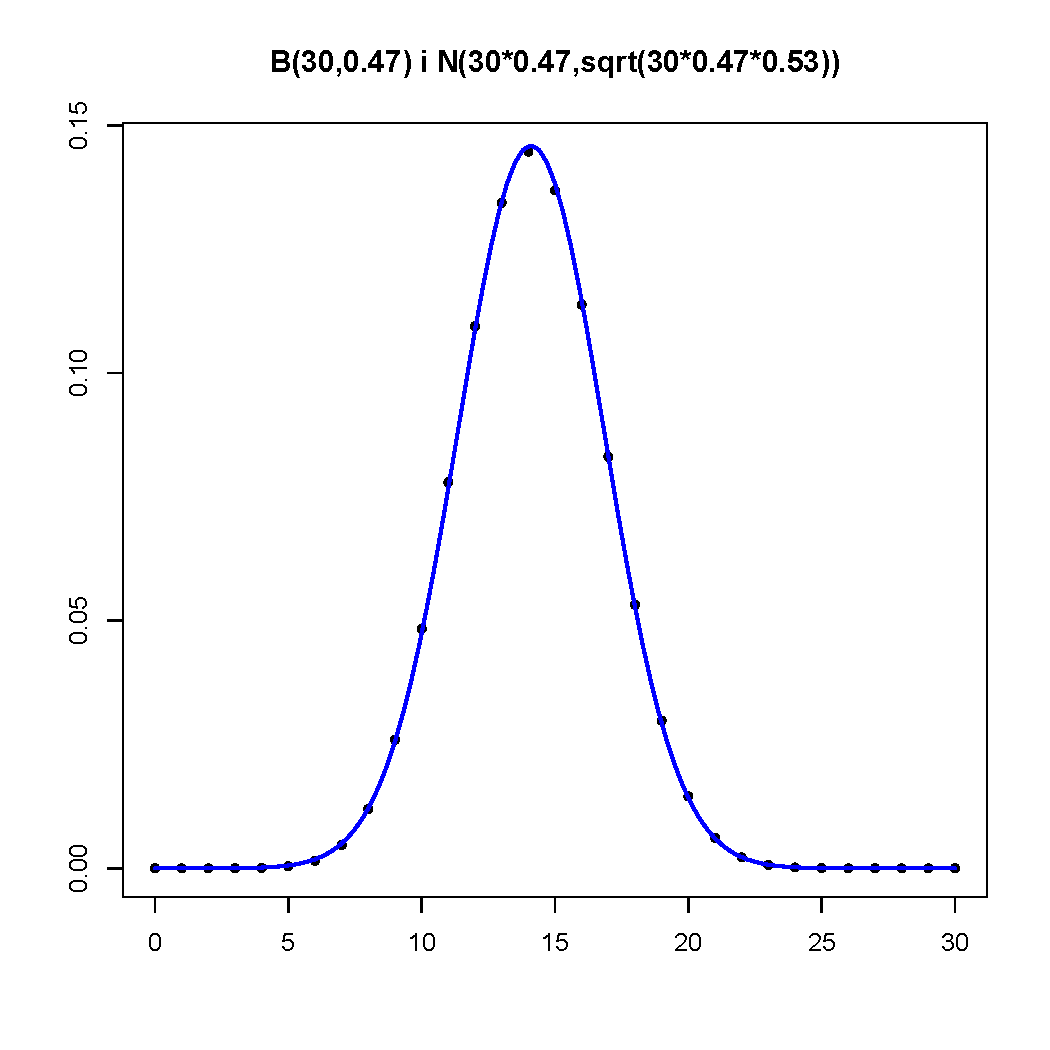
\includegraphics[width=0.58\linewidth]{normvsbin}
\end{center}


\end{frame}


\begin{frame}
\frametitle{Aproximació d'una binomial per una normal}
\vspace*{-2ex}

\begin{teorema}
Sigui  $X$ una v.a. $B(n,p)$, amb $n$ gran i $p$ que no estigui prop de 0 o 1. Sigui $Y$ una v.a. $N(np,\sqrt{npq})$. Aleshores 
$$
P(X=k)\approx  P\left(k-0.5\leq Y\leq k+0.5\right)
$$
\end{teorema}
De la suma $\pm 0.5$ per corregir l'efecte que té aproximar una v.a. discreta per una contínua se'n diu \emph{correcció de continuïtat de Fisher}.
\medskip

Hi ha diverses heurístiques per decidir què vol dir ``$n$ gran i $p$ no a prop de 0 o 1''. Per exemple: $$n\geq 20, np\geq 10\mbox{ i }n(1-p)\geq 10$$

\end{frame}

\begin{frame}[fragile]
\frametitle{Aproximació d'una binomial per una normal}
\vspace*{-1ex}

Sigui $X\sim B(30,0.47)$: $\mu\!=\!30\!\cdot\! 0.47$ i $\sigma\!=\!\sqrt{30\!\cdot\! 0.47\!\cdot\! 0.53}$
{\footnotesize \begin{verbatim}
> dbinom(13,30,0.47)
[1] 0.134361
> PY=function(x){pnorm(x,30*0.47,sqrt(30*0.47*0.53))}
> PY(13.5)-PY(12.5)
[1] 0.1339606
\end{verbatim}
}
\vspace*{-5ex}

\begin{center}
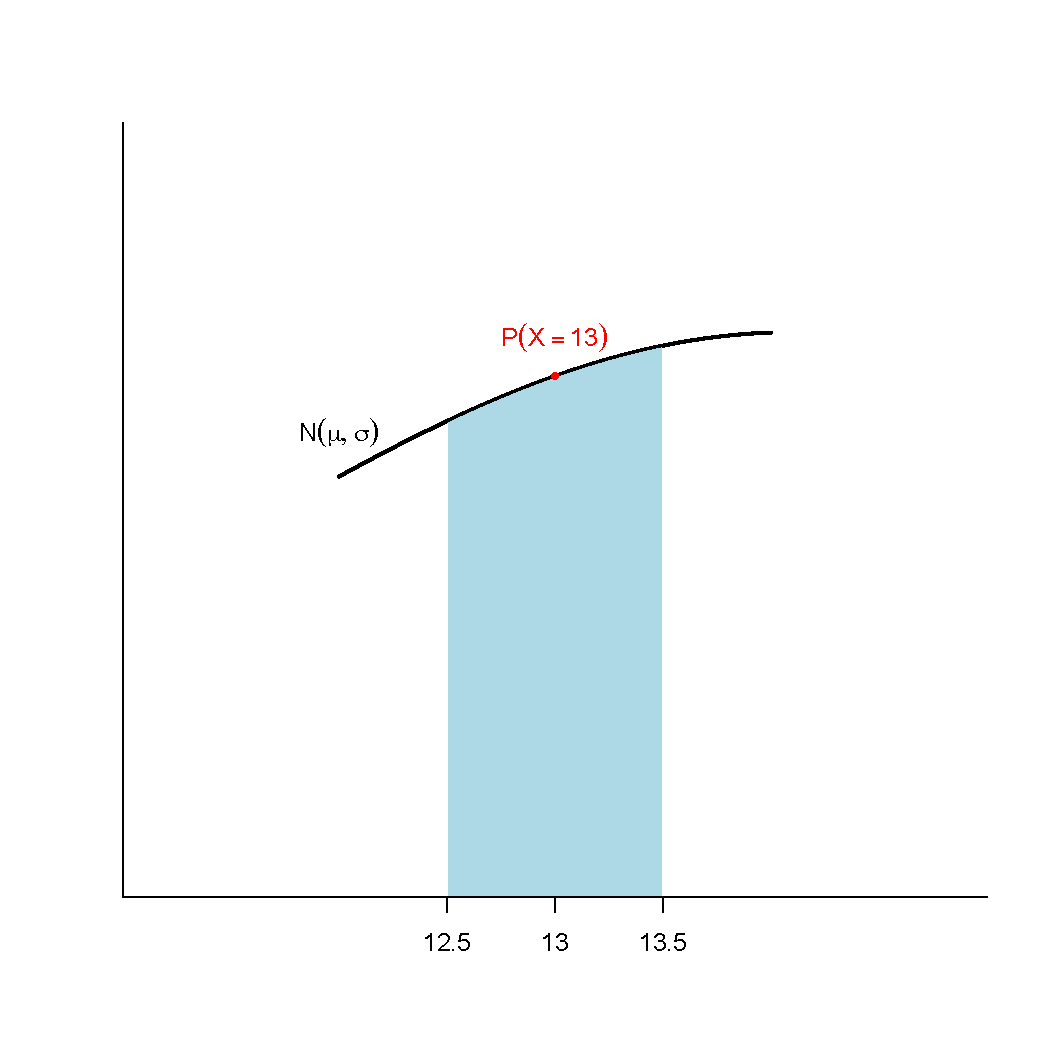
\includegraphics[width=0.6\linewidth]{binomvsnorm1}
\end{center}



\end{frame}



\begin{frame}
\frametitle{Aproximació d'una binomial per una normal}
\vspace*{-2ex}

Si $X$ és una v.a. $B(n,p)$ amb $n$ gran i $p$ que no estigui prop de 0 o 1,
$$
\frac{X-E(X)}{\sqrt{Var(X)}}=\frac{X-np}{\sqrt{npq}}
$$
s'aproxima per una normal estàndard $Z$:
$$
P(X=k) \approx P\left(\frac{k-0.5-np}{\sqrt{npq}}\leq Z \leq \frac{k+0.5-np}{\sqrt{npq}}\right)
$$


\end{frame}









\begin{frame}
\frametitle{Aproximació d'una binomial per una normal}

Si $X$ és una v.a. $B(n,p)$ amb $n$ gran i $p$ que no estigui prop de 0 o 1, i $Z$ és una v.a. normal estàndard:



$$
\begin{array}{l}
P(X\leq k)  \displaystyle\approx P\left(Z \leq
\frac{{k+0.5-np}}{\sqrt{npq}}\right)\\[3ex]
P(X\geq k)  \displaystyle\approx P\left(
\frac{{k-0.5-np}}{\sqrt{npq}}\leq Z\right)\\[3ex]
P(a\leq X\leq b) \displaystyle\approx
P\left(\frac{a-0.5-np}{\sqrt{npq}}\leq Z \leq
\frac{b+0.5-np}{\sqrt{npq}}\right)
\end{array}
$$
\end{frame}




\begin{frame}[fragile]
\frametitle{Exemple}
\blue{Llençam 100 vegades una moneda amb probabilitat de cara $\frac{1}{2}$.
Probabilitat de treure entre 40 i 49 cares?}
\bigskip

 $X$=nombre de cares en 100 llançaments d'una moneda
 \medskip
 
$X$  és $B(100,0.5)$
 \medskip
 
 
 
 Demanen $P(40\leq X\leq 49)$
 \medskip

\begin{verbatim}
> pbinom(49,100,0.5)-pbinom(39,100,0.5)
[1] 0.4426053
\end{verbatim}
\end{frame}


\begin{frame}
\frametitle{Exemple}
\vspace*{-1ex}

I si no tenim {\tt R}? Podem emprar la taula de $N(0,1)$:\medskip

$X\sim B(100,0.5)\Rightarrow E(X)=np=50,\ \sigma_{X}=\sqrt{npq}=5$
\medskip

$Z=\dfrac{X-50}{5}\sim N(0,1)$

$$
\begin{array}{l}
P(40\leq X\leq 49) \\ \displaystyle \qquad \approx  P\left(\frac{40-0.5-50}{5}\leq Z\leq
    \frac{49+0.5-50}{5}\right) \\[2ex] \displaystyle 
\qquad =  P(-2.1\leq Z\leq -0.1)\\[1ex]\displaystyle 
\qquad =
    F_{Z}(-0.1)-  F_{Z}(-2.1) \\[1ex] \displaystyle 
\qquad =    1-F_{Z}(0.1)-1+F_{Z}(2.1)\\[1ex] \displaystyle 
\qquad =
F_{Z}(2.1)-F_{Z}(0.1) = 0.9821-0.5398=0.4423
\end{array}
$$
\end{frame}



\end{document}





%\end{frame}
%\begin{frame}[fragile]
%\frametitle{Exemple}
%\vspace*{-1cm}
%
%$$
%\begin{array}{l}
%P(X=37) = P(37\leq X\leq 37) \\ \displaystyle \qquad \approx   P\left(\frac{37-0.5-50}{5}\leq Z\leq\frac{37+0.5-50}{5}\right)  \\ \displaystyle \qquad =   P\left(-\frac{13.5}{5}\leq Z\leq -\frac{12.5}{5}\right)  \\ \displaystyle \qquad = F_{Z}\left(-\frac{13.5}{5}\right)-F_{Z}\left(-\frac{12.5}{5}\right)  \\ \displaystyle \qquad =   F_{Z}(-2.5)-F_{Z}(-2.7) \\ \displaystyle \qquad =0.0062-0.0035=0.0027
%\end{array}
%$$
%\begin{verbatim}
%> dbinom(37,100,0.5)
%[1] 0.002697928
%\end{verbatim}
%\end{frame}
%
%\begin{frame}[fragile]
%\frametitle{Exemple}
%
%
%$$
%\begin{array}{l}
%\displaystyle P(X\leq 50)  \approx P\left(Z\leq \frac{50+0.5-50}{5}\right) \\[2ex] \displaystyle \qquad =P(Z\leq
%0.5)=F_{Z}(0.1)=0.5398
%\end{array}
%$$
%
%\begin{verbatim}
%> pbinom(50,100,0.5)
%[1] 0.5397946
%\end{verbatim}
%
%\end{frame}

\begin{frame}
\frametitle{Aproximació d'una Poisson per una normal}
\vspace*{-1ex}

Sigui  $X$ una v.a. $Po(\lambda)$, per tant $E(X)=Var(X)=\lambda$
\medskip

Si $\lambda$ és gran, aleshores $X$ és aproximadament $N(\lambda,\sqrt{\lambda})$
\vspace*{-1ex}

\begin{center}
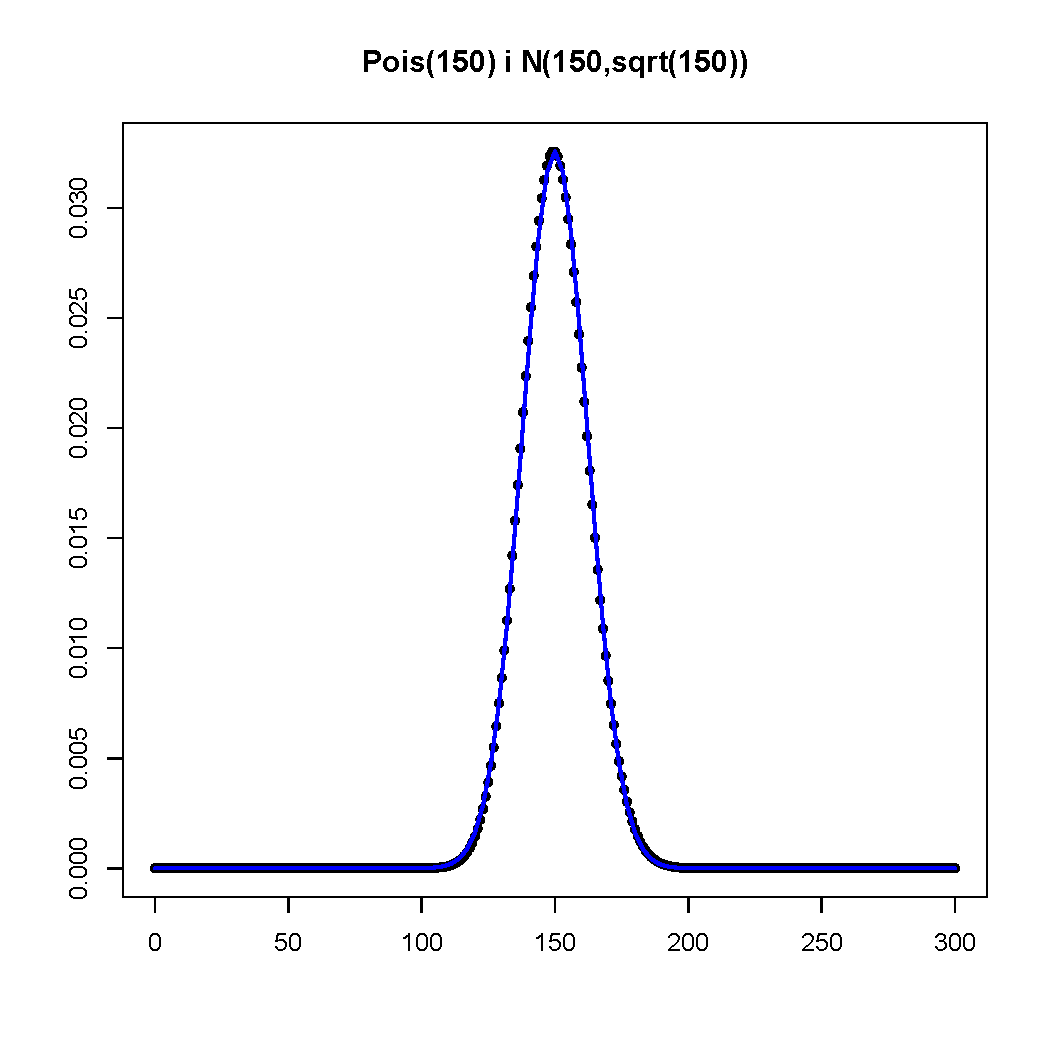
\includegraphics[width=0.6\linewidth]{poisvsnormal1}
\end{center}
\vspace*{-1cm}

Aquesta aproximació no és tan bona com a les binomials
\end{frame}


\begin{frame}



\frametitle{Aproximació d'una Poisson per una normal}


\begin{teorema}
Sigui  $X$ una v.a. $Po(\lambda)$, amb $\lambda$ gran. Sigui $Y$ una v.a. $N(\lambda,\sqrt{\lambda})$ (recordau que $E(X)\!=\!Var(X)\!=\!\lambda$). Llavors 
$$
P(X=k)\approx  P\left(k-0.5\leq Y\leq k+0.5\right)
$$
\end{teorema}
Per tant, si $X$ és una v.a. $Po(\lambda)$ amb $\lambda$ gran,
$$
\frac{X-\lambda}{\sqrt{\lambda}}
$$
s'aproxima per una normal estàndard $Z$, amb el sentit anterior
$$
P(X=k) \approx P\left(\dfrac{k-0.5-\lambda}{\sqrt{\lambda}}
\leq Z \leq \dfrac{k+0.5-\lambda}{\sqrt{\lambda}}\right)
$$

\end{frame}










